%%%%%%%%%%%%%%%%%%%%%%%%%%%%%%%%%%%%%%%%%%%%%%%%%%%%%%%%
%%%%                                              %%%%%%
%%%%  Author: Peter Wilson                        %%%%%%
%%%%                                              %%%%%%
%%%%  Background of shells                        %%%%%%
%%%%                                              %%%%%%
%%%%%%%%%%%%%%%%%%%%%%%%%%%%%%%%%%%%%%%%%%%%%%%%%%%%%%%%


%fref generates automatically the respective abreviation/word in the text for the reference. You just have to define a label starting with the respective keyword.
%english: chap, sec, fig, eq, app
%deutsch: chap/kap, abs, abb, gl, anh
%see http://ctan.space-pro.be/tex-archive/macros/latex/contrib/fancyref/fancyref.pdf for more \section

%\onehalfspacing
%\setlength{\belowcaptionskip}{-17pt}

\chapter{Shell finite elements - revised 2}
\label{chap:chapter_2}

\renewcommand{\Thema}{Shell finite elements}

\lettrine[lines=2]{T}{he} employment of shell structures is ubiquitous throughout both nature and the built environment. Eggs, nuts, blood vessels and cell walls are examples of shell designs being the result of structural optimisation via natural evolution over millennia. It is no doubt that man drew inspiration from the optimal natural shell design and realised the efficacy of the shell structure, with the harnessing of these principles culminating in the pre-eminent Roman Pantheon (126).  Throughout time, as the understanding of shell structures increased, so did their prevalence, leading to notable structures such as the Hagia Sophia (537), Notre Dame (1345) and St. Peter's Basilica (1626). Indeed, the efficiency of shell structures lies in their high in-plane (membrane) load carrying capacity in slender low-weight constructions. The membrane action serves to stress all fibres approximately equally in the cross section, realising the full mechanical performance of the structure. Contrasting this, shells are incredibly sensitive to a variety of effects such as imperfections, bending, transverse normal forces and support conditions, leading to significant compromise of the membrane structural performance and possibly manifesting in catastrophic failure. To examine one such sensitivity, bending actions result in a non-uniform stressing of material fibres over the cross section, with the outer fibres stressed significantly more than those closer to the neutral axis. Consequently, the limit of the structure in bending is realised when only the outer-most fibre fails instead of the entire cross section of fibres failing under membrane action. This basic example offers a snapshot of the stellar performance of shells juxtaposed against their sensitivity to a multitude of conditions, earning them the title of the \textit{Prima Donna of structures} \cite{Ram16}.

\section{Structural modelling with shells}
Although shells present the opportunity of an optimally loaded structure, their delicate position in a sharply varying landscape of performance demands careful consideration of phenomena critical to the analysis undertaken. When this potentially volatile behaviour is held against the scientific ethos of \textit{everything should be made as simple as possible, but no simpler}, the arising tension is immediately recognized, one that can only be curtailed by an in depth knowledge of the working problem and shells themselves. Within the engineering design context of a particular scenario, there exists as many opportunities to reasonably reduce complexity as there are to incorrectly exclude critical phenomena. Typical structural modelling decisions such as: inclusion or exclusion of inertial and damping effects, non-linear or linear material models, large or small deformation assumptions and dimensional reduction are examples of broad brush strokes limiting the canvas of possibilities resolved. Focussing on the rendering of shells, the assumed underlying structural models  effectively scope and frame the domain of potential mechanical expressions for a system.

Inherent in the use of shells in structural models is the concept of dimensional reduction from 3 dimensions to 2 dimensions, relying on the assumption that one dimension (thickness) is significantly smaller than the other two (length and width). 

\begin{figure}[H]
	\centering
	\def\svgwidth{\columnwidth}
	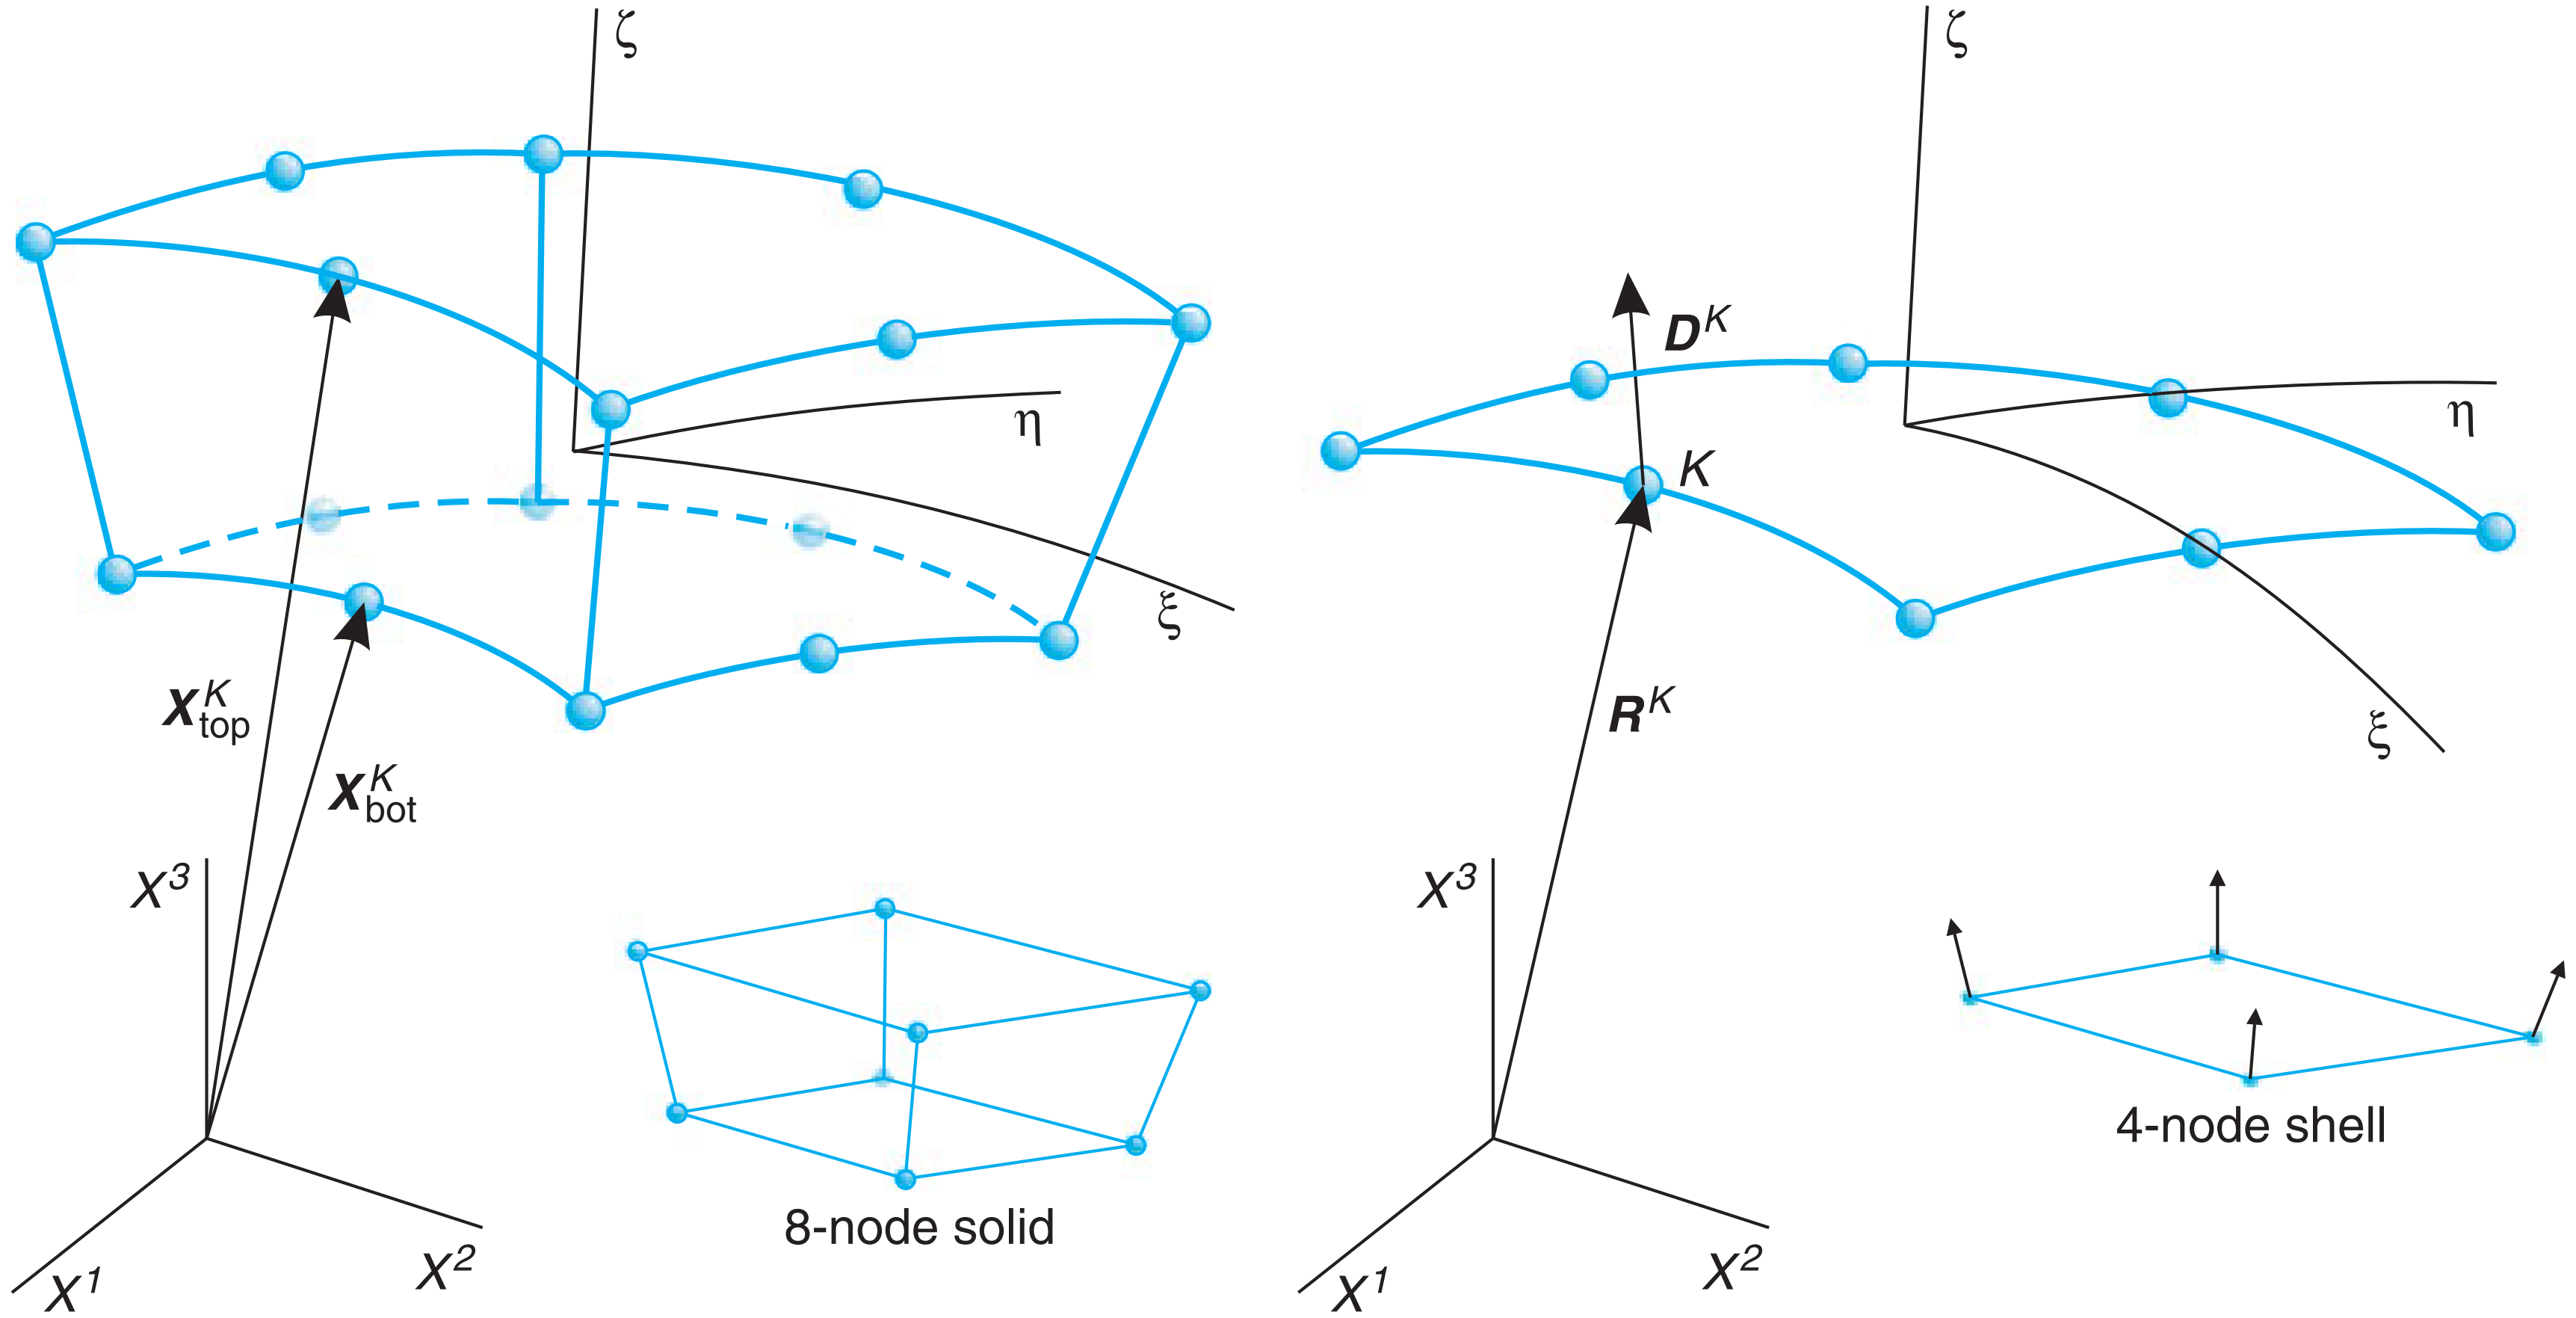
\includegraphics[width=12cm]{images/degenerateshell.png}
	\caption{Dimensional reduction of a solid to a shell \cite{BischLitBook04}}
	\label{dimReduction}
\end{figure}

Already, it is apparent that the through-thickness response of the shell now must be modelled instead of resolved, with the results now a function of the approximation employed. This apparent simplification promptly begs a key question: what shall the model consider such that it is simple as possible, but not simpler? Can the thickness vary under deformation? Is the shell one uniform material or multi-layered? Is shear deformation of the thickness negligible or not? One may also impose far stricter modelling assumptions by only considering the bending or membrane behaviour of the shell. These common structural modelling decisions, amongst others, have yielded typical shell models.

\section{Shell models}

Commencing in the Renaissance and continuing into the present day, the mathematical development of shell models has facilitated the construction of increasingly elaborate shell structures. The main mathematically-based shell models considered in this work are illustrated below.

\begin{figure}[H]
	\centering
	\def\svgwidth{\columnwidth}
	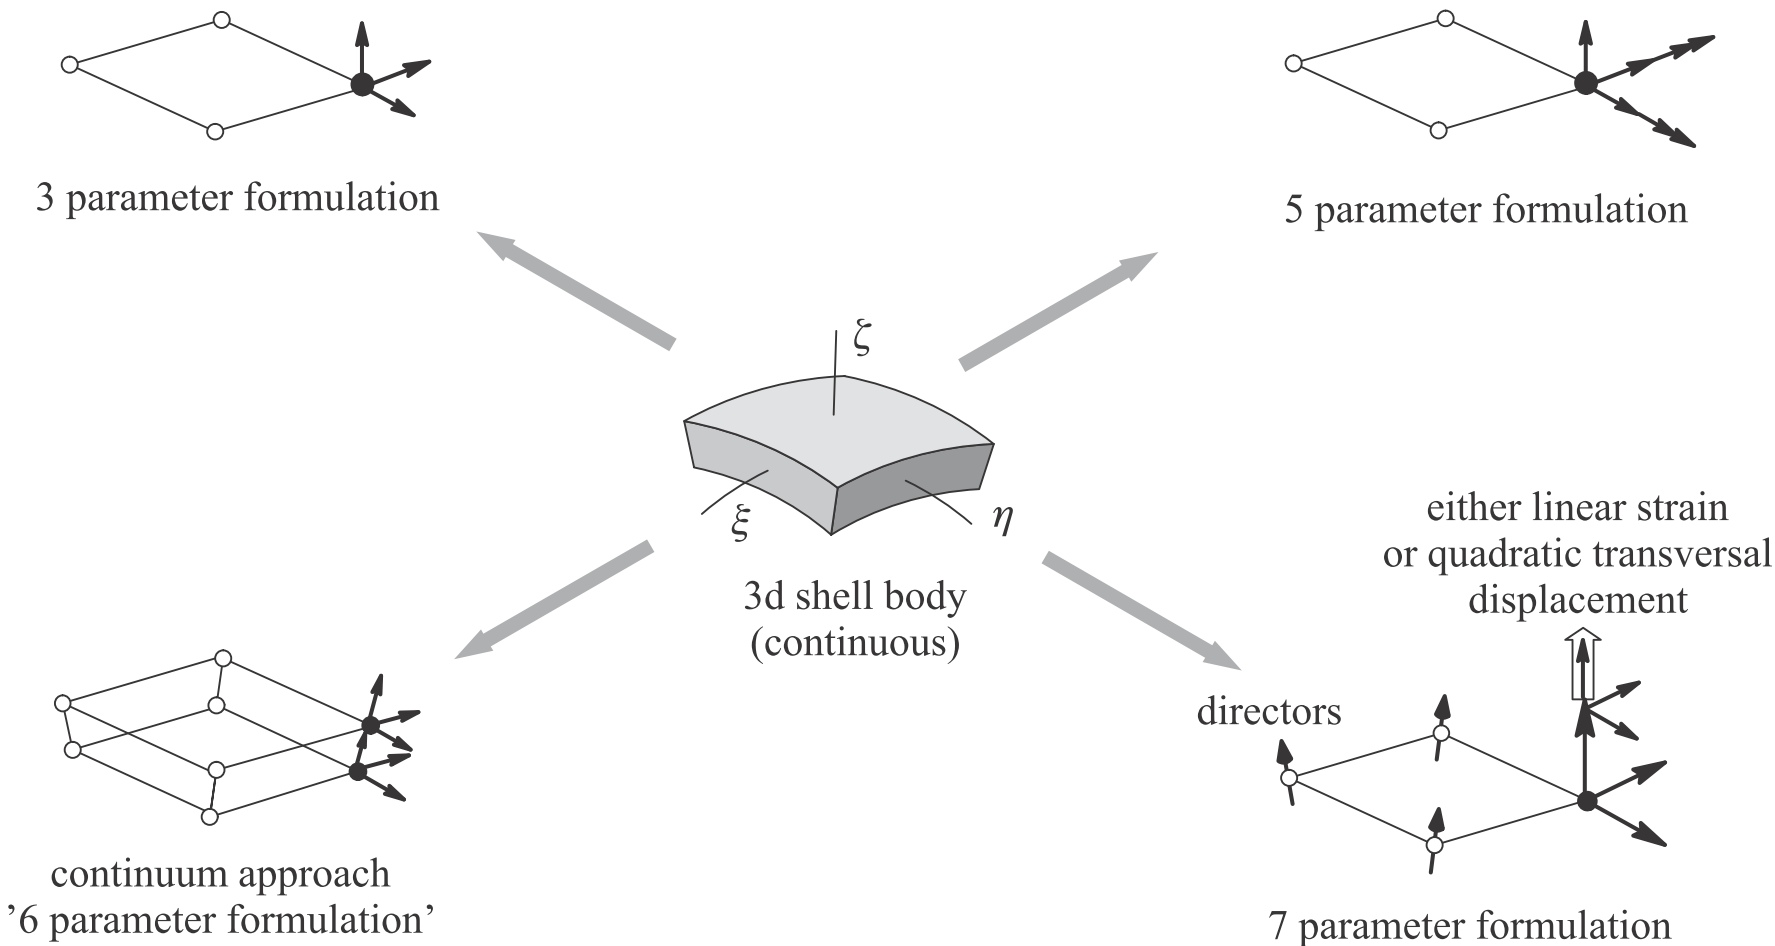
\includegraphics[width=12cm]{images/shellModels.png}
	\caption{Various shell models \cite{Wall2000}}
	\label{shellModels}
\end{figure}

Each of the shell models above are based on different assumptions and physics, which essentially act as a filter of what phenomena the structural model can resolve. These models, as well as the basic membrane model, will be briefly discussed in the following section (further details can be found in References \cite{BischLitBook04} \cite{RammLitBook04} and \cite{Echter13}). To gain further insight, high level formulations of the models are presented with a focus of the mathematical representation of key assumptions.  The follow figure illustrates the configurations and notation of the formulations. 

\begin{figure}[H]
	\centering
	\def\svgwidth{\columnwidth}
	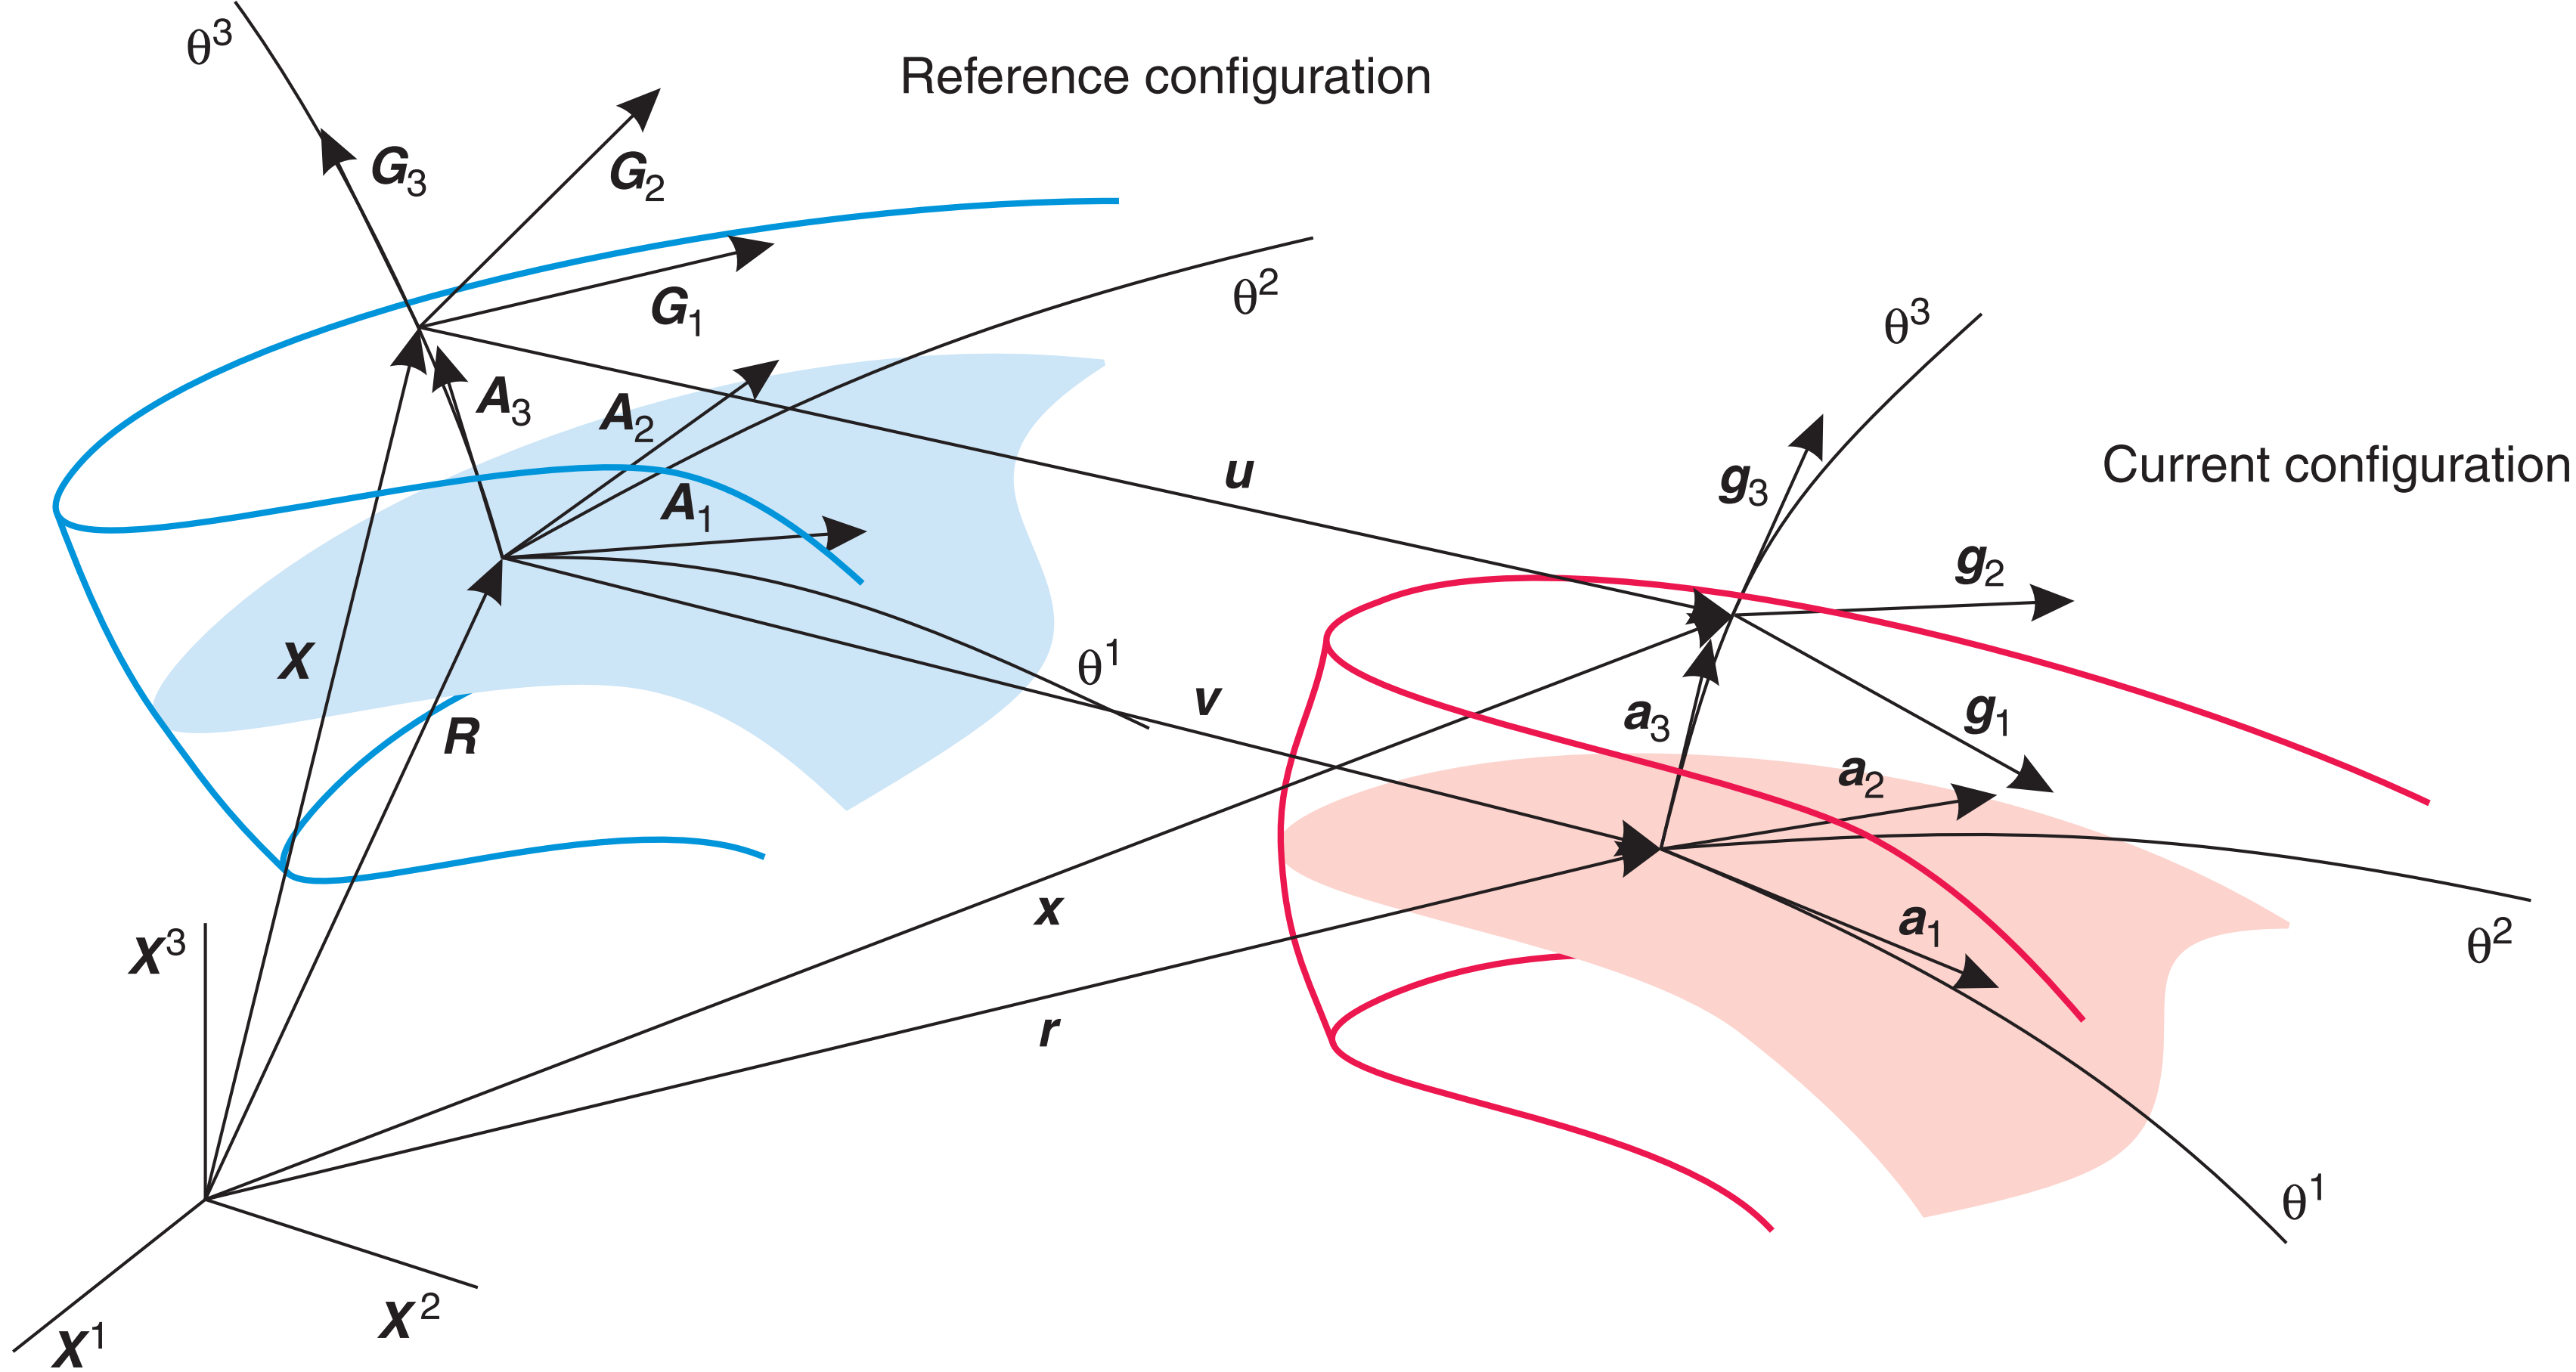
\includegraphics[width=12cm]{images/shellsconfig.png}
	\caption{Deformation, reference and current configuration \cite{BischLitBook04}}
	\label{shellsconfig}
\end{figure}

Quantities in the reference configuration are expressed in upper case while quantities in lower case are in the deformed configuration. The reference shell mid-plane $\theta^3 = 0$ position vector of a point is denoted $\mathbf{R}$, while an arbitrary point is denoted $\mathbf{X}$. Correspondingly, base vectors on the mid-plane are denoted $\mathbf{A}_i$ and $\mathbf{a}_i$ while $\mathbf{G}_i$ and $\mathbf{g}_i$ denote arbitrary base vectors. It is noted that Einstein notation is employed here, with Latin characters corresponding to summation over three dimensions while Greek characters sum over two dimensions. Lastly, $\mathbf{v}$ and $\mathbf{u}$ indicate displacements on the mid-plane and an arbitrary location respectively.

\subsection{Membrane model}

Despite not truly being a shell model, the membrane model is the simplest model available as it completely ignores bending behaviour. Thus, the structural behaviour of the whole element is described by in plane components. Typically it is assumed that all stress and strain components are constant over the thickness. A key model choice is the specification of either plane stress or plane strain behaviour which is implemented in material matrix.

Commencing a high level formulation of the membrane model, the assumption of constant strain and stress components over the thickness allows collapsing the body into an infinitely thin shell. Thus thickness can be ignored in the position vectors.

\begin{equation} 
\mathbf{X} = \mathbf{R}\ ,
\hspace{10mm}
\mathbf{x} = \mathbf{r}\ ,
\hspace{10mm}
\mathbf{r} = \mathbf{R} + \mathbf{v}
\label{eqsmem1a}
\end{equation}

Using the notation of $(\ )_{,\alpha} = \frac{\partial(\ )}{\partial	\alpha}$ and explicitly writing the base vectors of the coordinate system yields:

\begin{equation} 
\mathbf{A}_\alpha  = \mathbf{R}_{,\alpha} =  \mathbf{X}_{,\alpha}
\ ,
\hspace{10mm}
\mathbf{a}_\alpha  = \mathbf{r}_{,\alpha} = \mathbf{A}_\alpha + \mathbf{v}_{,\alpha}
\label{eqsmem1b}
\end{equation}

Considering the metrics of the reference and deformed configuration, the in-plane Green-Lagrange strain components read:

\begin{equation} 
\epsilon_{\alpha\beta} = \frac{1}{2}
(a_{\alpha\beta} - A_{\alpha\beta})
\hspace{10mm}
with
\hspace{10mm}
a_{\alpha\beta} = \mathbf{a}_\alpha \cdot \mathbf{a}_\beta
\hspace{10mm}
A_{\alpha\beta} = \mathbf{A}_\alpha \cdot \mathbf{A}_\beta
\label{eqsmem2}
\end{equation}

Corresponding to the membrane assumptions, all out of plane strain components are 0.

\begin{equation} 
\epsilon_{3i} = 0
\label{eqsmem3}
\end{equation}

At this point, one notices that all strain terms are completely contained within the two in-plane mid-surface displacements $\mathbf{v}_\alpha$.

By introducing the elasticity tensor $\mathbf{C}_0$ (typically plane stress) the stress components can be recovered from the strains.

\begin{equation} 
\sigma^{\alpha\beta} = C_0^{\alpha\beta\gamma\delta} \epsilon_{\gamma\delta}
\label{eqsmem4}
\end{equation}

With stresses and strains determined, the internal and a generalised (where $\mathbf{f}$ is a generalised traction vector and $\delta \mathbf{v}$ are virtual displacements) external virtual work can be expressed:

\begin{equation} 
-\delta\Pi_{int} = 
\int_\Omega
\boldsymbol{\epsilon}
:
\mathbf{C}_{mem}
:
\delta \boldsymbol{\epsilon}\ 
d \Omega\ ,
\hspace{10mm}
\delta\Pi_{ext} = \int_\Omega
\mathbf{f}^T
\delta  \mathbf{v}\ 
d \Omega
\label{eqsmem5}
\end{equation}

%Condensing to vector notation the above yields:
%
%\begin{equation} 
% \boldsymbol{\epsilon} =  \begin{pmatrix}
%  \epsilon_{xx} \\
%  \epsilon_{yy} \\
%  2\epsilon_{xy} \\
% \end{pmatrix} 
% \hspace{10mm}
% \mathbf{C}_0 = \frac{E}{1-\nu^2} \bar{\mathbf{C}} = \frac{E}{1-\nu^2}
% \begin{pmatrix}
%  1 & 0 & 0 \\
%   0 & 1 & 0 \\
%    0 & 0 & \frac{1-\nu}{2}
% \end{pmatrix} 
%\label{eqsmem7}
%\end{equation}

%\begin{equation} 
%\delta\Pi_{ext} = \int_\Omega
% \mathbf{f}^T
%\delta  \mathbf{v}\ 
%d \Omega
%\label{eqsmem7}
%\end{equation}

It's apparent that the internal work is composed solely of in-plane action, corresponding to the general descriptive assumptions of the membrane model above. By extension, it can be understood that the membrane model provides no resistance to out of plane action. Thus, unless the membrane-modelled structure is pre-stressed, the system will be rendered singular under out of plane loads. This lack of out of plane stiffness can also lead to buckling under compressive stresses. Considering the reduced phenomena that the membrane model can resolve, it is crucial to understand the critical physics of the system before employing it.

\subsection{3 parameter model: Kirchhoff-Love shell}

The first actual shell model considered is the 3 parameter model, often referred to as the Kirchhoff-Love (KL) shell. This model includes all membrane considerations, but also describes bending behaviour too. The bending behaviour is constrained to a description similar to the Bernoulli beam: shell directors across the thickness remain straight and normal to the mid-surface. Graphically, this is represented in the following figure:

\begin{figure}[H]
	\centering
	\def\svgwidth{\columnwidth}
	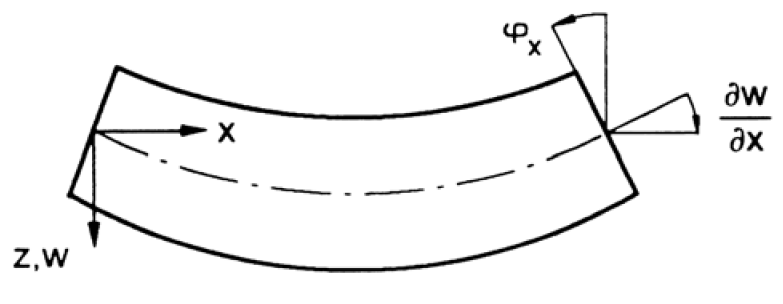
\includegraphics[width=8cm]{images/bernoullie.png}
	\caption{Kirchhoff-Love shell kinematics \cite{Bletz16}}
	\label{thinshellkine1}
\end{figure}

A consequence of the above kinematics is that this model ignores transverse shear strains. Thus, the applicability of the 3 parameter model is clearly limited to thin plates in the range of $\frac{1}{5} < \frac{l}{t} < \frac{1}{50}$ where transverse deformations are negligible. Similar to the membrane model, thickness deformation is ignored.

Establishing the geometry of the KL shell requires incorporation of the shell director along $\theta^3$ in the reference $\mathbf{D}$ and deformed configuration $\mathbf{d}$.

\begin{equation} 
\mathbf{X} = \mathbf{R} + \theta^3 \mathbf{D}\ ,
\hspace{10mm}
\mathbf{x} = \mathbf{r} + \theta^3 \mathbf{d}\ ,
\hspace{10mm}
\mathbf{r} = \mathbf{R} + \mathbf{v}\ ,
\hspace{10mm}
\mathbf{d} = \boldsymbol{\Lambda}  \mathbf{D}
\label{eqskt1}
\end{equation}

The above equation enforces the KL condition of a straight director with the linear description of $\theta^3 \mathbf{d}$. $\boldsymbol{\Lambda}$ is a rotation tensor composed of two independent rotation parameters $\beta^\alpha$ relating the reference and deformed directors to each other. In a Cartesian frame the linearised rotation components are: $\beta^1 = \mathbf{v}_{3,2}$ and $\beta^2 = -\mathbf{v}_{3,1}$ \cite{BischLitBook04}.

The displacement is thus expressed:

\begin{equation} 
\mathbf{u} = \mathbf{x} - \mathbf{X}
=
\mathbf{v} + \theta^3 (\boldsymbol{\Lambda} - \mathbf{G}) \mathbf{D}
=
\mathbf{v} + \theta^3 \mathbf{d}
\label{eqskt2}
\end{equation}

!!!!!!!!!!!!!!!!!!!!!!!!!!!!!
Gotta figure out lamda - G = lamda
!!!!!!!!!!!!!!!!!!!!!!!!!!!!! \\

The KT requirement of the director being normal to the mid surface is expressed via the following dot product:

\begin{equation} 
\mathbf{d} \cdot \mathbf{r}_{,\alpha}
=
(\boldsymbol{\Lambda} \mathbf{D}) \cdot (\mathbf{A}_\alpha + \mathbf{v}_{,\alpha})
=
0
\label{eqskt3}
\end{equation}

Explicitly writing the base vectors of the coordinate system:

\begin{equation} 
\mathbf{A}_\alpha  = \mathbf{R}_{,\alpha}
\hspace{10mm}
\mathbf{a}_\alpha  = \mathbf{r}_{,\alpha} = \mathbf{A}_\alpha + \mathbf{v}_{,\alpha}
\label{eqskt4}
\end{equation}

Eqn \eqref{eqskt3}, requiring the director to be normal to the mid-surface, is guaranteed by employing cross products of the base vectors to construct the directors:

\begin{equation} 
\mathbf{D} = \frac{\mathbf{A}_1 \times \mathbf{A}_2}
{\lvert \lvert \mathbf{A}_1 \times \mathbf{A}_2 \rvert \rvert}
= \mathbf{A}_3\ ,
\hspace{10mm}
\mathbf{d} = \frac{\mathbf{a}_1 \times \mathbf{a}_2}
{\lvert \lvert \mathbf{a}_1 \times \mathbf{a}_2 \rvert \rvert}
= \mathbf{a}_3\ ,
\label{eqskt5}
\end{equation}

As the KT model considers bending, which is related to curvature, the second fundamental form of the system is defined in the reference and deformed configuration:

\begin{equation} 
B_{\alpha \beta} = \frac{1}{2} 
( 
\mathbf{A}_\alpha \cdot \mathbf{A}_{3,\beta} 
+
\mathbf{A}_\beta \cdot \mathbf{A}_{3,\alpha}
)
=
\mathbf{A}_\alpha \cdot \mathbf{A}_{3,\beta}
=
\mathbf{A}_\alpha \cdot \mathbf{D}_{,\beta}
\label{eqskt6}
\end{equation}

\begin{equation} 
b_{\alpha \beta} = \frac{1}{2} 
( 
\mathbf{a}_\alpha \cdot \mathbf{a}_{3,\beta} 
+
\mathbf{a}_\beta \cdot \mathbf{a}_{3,\alpha}
)
=
\mathbf{a}_\alpha \cdot \mathbf{a}_{3,\beta}
=
(\mathbf{A}_\alpha + \mathbf{v}_{,\alpha}) 
\cdot 
\Bigg({
	\frac{    (\mathbf{A}_1 + \mathbf{v}_{,1})  \times (\mathbf{A}_2 + \mathbf{v}_{,2})    }
	{\lvert \lvert  (\mathbf{A}_1 + \mathbf{v}_{,1})  \times (\mathbf{A}_2 + \mathbf{v}_{,2})   \rvert \rvert}
}\Bigg)_{,\beta}
\label{eqskt7}
\end{equation}

Contrasting with the membrane model, the KT strain tensor components now include linearly varying terms corresponding to bending phenomena:

\begin{equation} 
E_{\alpha \beta}
= \frac{1}{2}
(a_{\alpha\beta} - A_{\alpha\beta})
+
\theta^3 (b_{\alpha\beta} - B_{\alpha\beta})
=
\epsilon_{\alpha \beta} + \theta^3 \kappa_{\alpha \beta}
\label{eqskt8}
\end{equation}

According to the KT assumptions all out of plane strains are zero.

\begin{equation} 
E_{3i} = \epsilon_{3i} = \kappa_{3i} = 0
\label{eqskt81}
\end{equation}

Studying the strain components, especially the deformed second fundamental form, reveals that there are now 3 midplane displacements $\mathbf{v}_i$ involved in the description of the KT shell model, hence the name 3 parameter model. 

Combining the above developments, and assuming the same general external work as equation \eqref{eqsmem5}, the internal virtual work can be presented:

\begin{equation} 
-\delta\Pi_{int} = 
\int_\Omega
\boldsymbol{\epsilon}
:
\mathbf{C}_{mem}
:
\delta \boldsymbol{\epsilon}\ d \Omega\ 
+
\int_\Omega
\boldsymbol{\kappa}
:
\mathbf{C}_{bend}
:
\delta \boldsymbol{\kappa}\ 
d \Omega
\label{eqskt9}
\end{equation}

The internal work equation illustrates the 3 parameter model considers in-plane membrane behaviour as well as the additional bending behaviour related to the second integral. Furthermore, under the condition of homogeneous linear material models the membrane and bending behaviour of the model are uncoupled. Due to the kinematics of the 3 parameter model (directors remain straight and normal, no transverse shear strains), it can correctly resolve analyses as shell thicknesses approach zero. This is in contrast the to 5 parameter model, which exhibits significant shear locking. Despite this, a pure rendition of the 3 parameter model is not commonly seen in practical FEM due to the required $C_1$ continuity at element boundaries (arising from rotations expressed as derivatives of transverse displacement) and the additional complication of effective shear forces on boundaries \cite{BischLitBook04}.

\subsection{5 parameter model: Reissner-Mindlin shell}

By relaxing the assumptions made in the 3 parameter shell model, the Reissner-Mindlin (RM) 5 parameter shell model can be derived. This model includes both membrane and bending action. While the KL model required that the shell directors remain normal to the mid-surface, the RM model relaxes this, analogous to the relationship between Bernoulli and Timoshenko beam models. Graphically, this is represented in the following figure:

\begin{figure}[H]
	\centering
	\def\svgwidth{\columnwidth}
	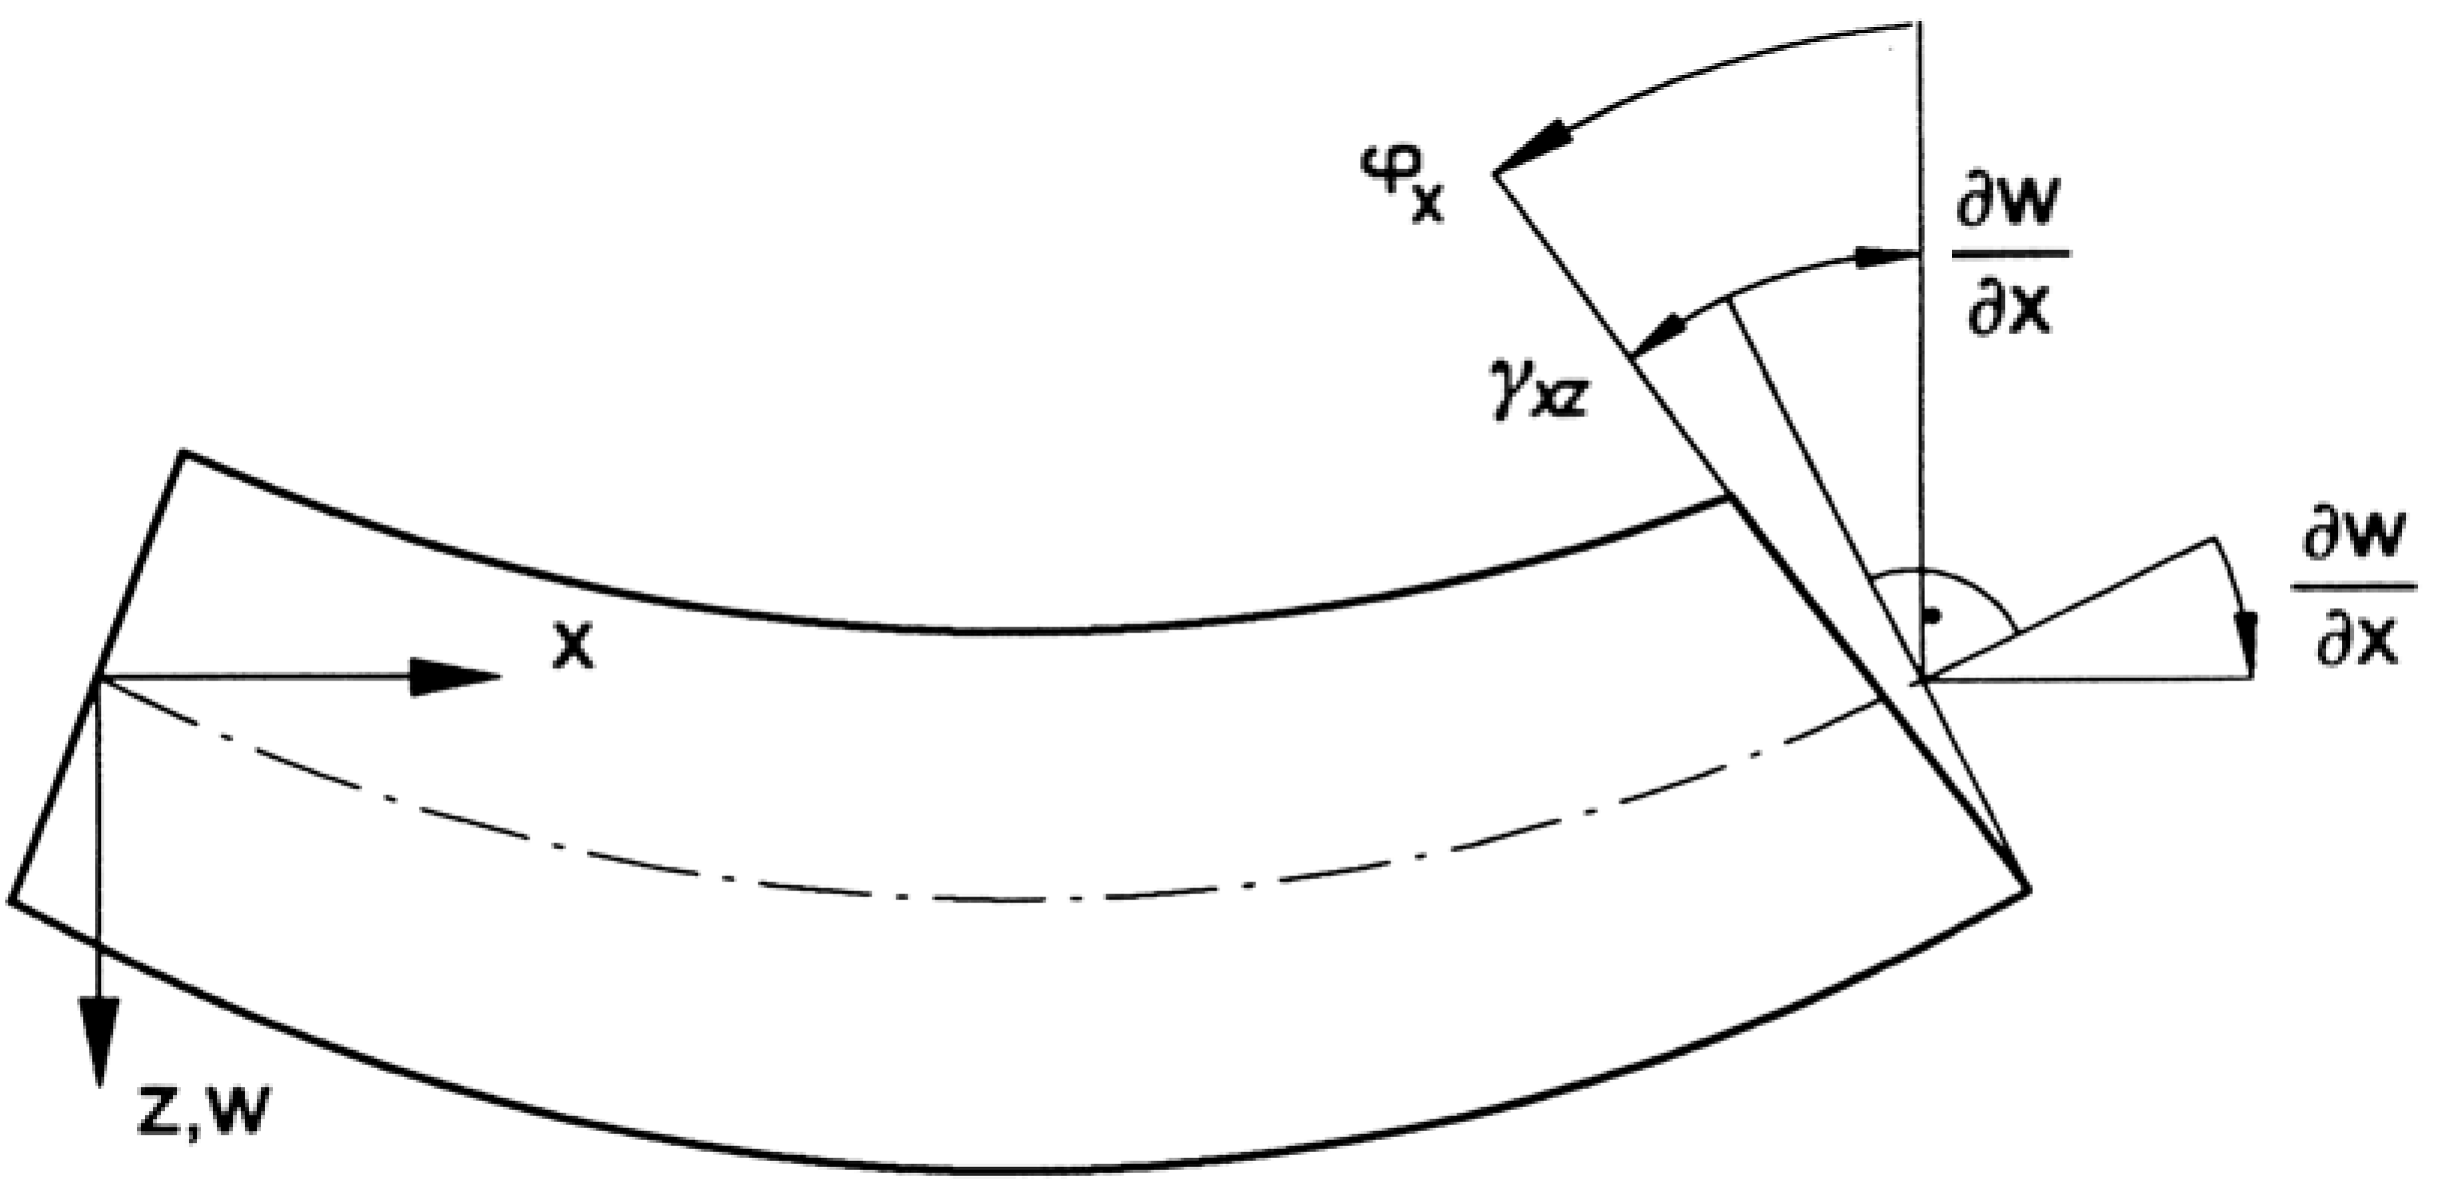
\includegraphics[width=8cm]{images/timoshenkobeam.png}
	\caption{Reissner-Mindlin shell kinematics \cite{Bletz16}}
	\label{thickshellkine1}
\end{figure}

Studying the above kinematics confirms this model now considers transverse shear strains, limiting the range of validity of this model to thick plates $\frac{1}{5} < \frac{l}{t} < \frac{1}{10}$ where transverse deformations are a key component of structural behaviour. Similar to the membrane and KL model, thickness deformation is ignored. 

The geometry of the RM model is established similar to the KL model:

\begin{equation} 
\mathbf{u} = \mathbf{x} - \mathbf{X}
=
\mathbf{v} + \theta^3 (\boldsymbol{\Lambda} - \mathbf{G}) \mathbf{D}
=
\mathbf{v} + \theta^3 \mathbf{d}
\label{eqsrm1}
\end{equation}

However, the strict requirement of maintaining the director remain normal to the mid-surface, as expressed in the KL theory equation \eqref{eqskt3}, is no longer enforced. Correspondingly, the rotation tensor $\boldsymbol{\Lambda}$ must now include 2 additional parameters related to these 2 introduced degrees of freedom.

The general strain components are expressed as:

\begin{equation} 
E_{\alpha \beta}
= \frac{1}{2}
(a_{\alpha\beta} - A_{\alpha\beta})
+
\theta^3 (b_{\alpha\beta} - B_{\alpha\beta})
=
\epsilon_{\alpha \beta} + \theta^3 \kappa_{\alpha \beta}
\label{eqsrm2}
\end{equation}

Once again it is noted the assumption of straight directors is enforced by the linear coupling of $\theta^3 \kappa_{\alpha \beta}$. Following the assumption of no thickness strain, it is seen:

\begin{equation} 
E_{33} = \epsilon_{33} = \kappa_{33} = 0
\label{eqsrm21}
\end{equation}

By relaxing the director normality requirements, additional transverse shear strains must be accounted for:

\begin{equation} 
E_{\alpha 3} = E_{3 \alpha}
= \frac{1}{2}
(a_{\alpha 3} - A_{\alpha 3})
=
\frac{1}{2} \gamma_{3\alpha}
\label{eqsrm3}
\end{equation}

The internal virtual work is therefore expressed as:

\begin{equation} 
-\delta\Pi_{int} =
\int_\Omega
\boldsymbol{\epsilon}
:
\mathbf{C}_{mem}
:
\delta \boldsymbol{\epsilon}\ d \Omega\ 
+
\int_\Omega
\boldsymbol{\kappa}
:
\mathbf{C}_{bend}
:
\delta \boldsymbol{\kappa}\ 
d \Omega\ 
+
\int_\Omega
\boldsymbol{\gamma}
:
\mathbf{C}_{shear}
:
\delta \boldsymbol{\gamma}\ 
d \Omega
\label{eqsrm4}
\end{equation}

%\begin{equation} 
% \boldsymbol{\epsilon} =  \begin{pmatrix}
%  \epsilon_{xx} \\
%  \epsilon_{yy} \\
%  \epsilon_{xy} \\
% \end{pmatrix} 
% \hspace{10mm}
% \boldsymbol{\kappa} =  \begin{pmatrix}
%  \kappa_{xx} \\
%  \kappa_{yy} \\
%  2\kappa_{xy} \\
% \end{pmatrix} 
%  \hspace{10mm}
%  \boldsymbol{\gamma} =  \begin{pmatrix}
%  \gamma_{xz} \\
%  \gamma_{yz} \\
% \end{pmatrix} 
%\label{eqsrm6}
%\end{equation}

The 3 integrals of the virtual work equation represent the membrane, bending and shear work components, corresponding to the phenomena this model resolves. Furthermore, all these components are decoupled from each other in flat shells with homogeneous linear material models. The consideration of transverse shear deformations in the kinematics render the model applicable to thick shells where these strains are not insignificant. Incorrectly applying this model to thin shells in FEM yields spurious results due to a phenomena called shear locking (discussed in section \ref{transverse_shear_locking}). Despite this disadvantage, the 5 parameter forms the basis of many shell elements often used in FEM thanks to the lower $C_0$ continuity required at element boundaries.

\subsection{7 parameter model}

The previously discussed models all operate under the assumption that the transverse normal strains are zero. The 7 parameter model considers thickness deformation by introducing additional free parameters. Only a brief overview of the 7 parameter model is offered here as shell elements in FEM, the focus of this work, are predominately based off 3 and 5 parameter based formulations. For further details refer Bischoff et al. \cite{BischLitBook04} and Ramm and Wall \cite{RammLitBook04}.

Intuitively, one may realise that shell behaviour including thickness change may be described by 6 parameters:  3 mid-surface displacements, 1 thickness change and 2 rotations.  However, thickness locking occurs under this regime due to a mismatch of a linearly varying normal thickness stress $\theta^{33}$ conjugated with a constant thickness strain $\epsilon_{33}$. Thus the 7th parameter is the enhancement of the through thickness strain $\epsilon_{33}$ to a linear field.

It's clear that the additional modelling power of the 7 parameter shell can resolve physics that lower parameter models can't. A prime example of this is the Eigenvalue spectra presented below:

\begin{figure}[H]
	\centering
	\def\svgwidth{\columnwidth}
	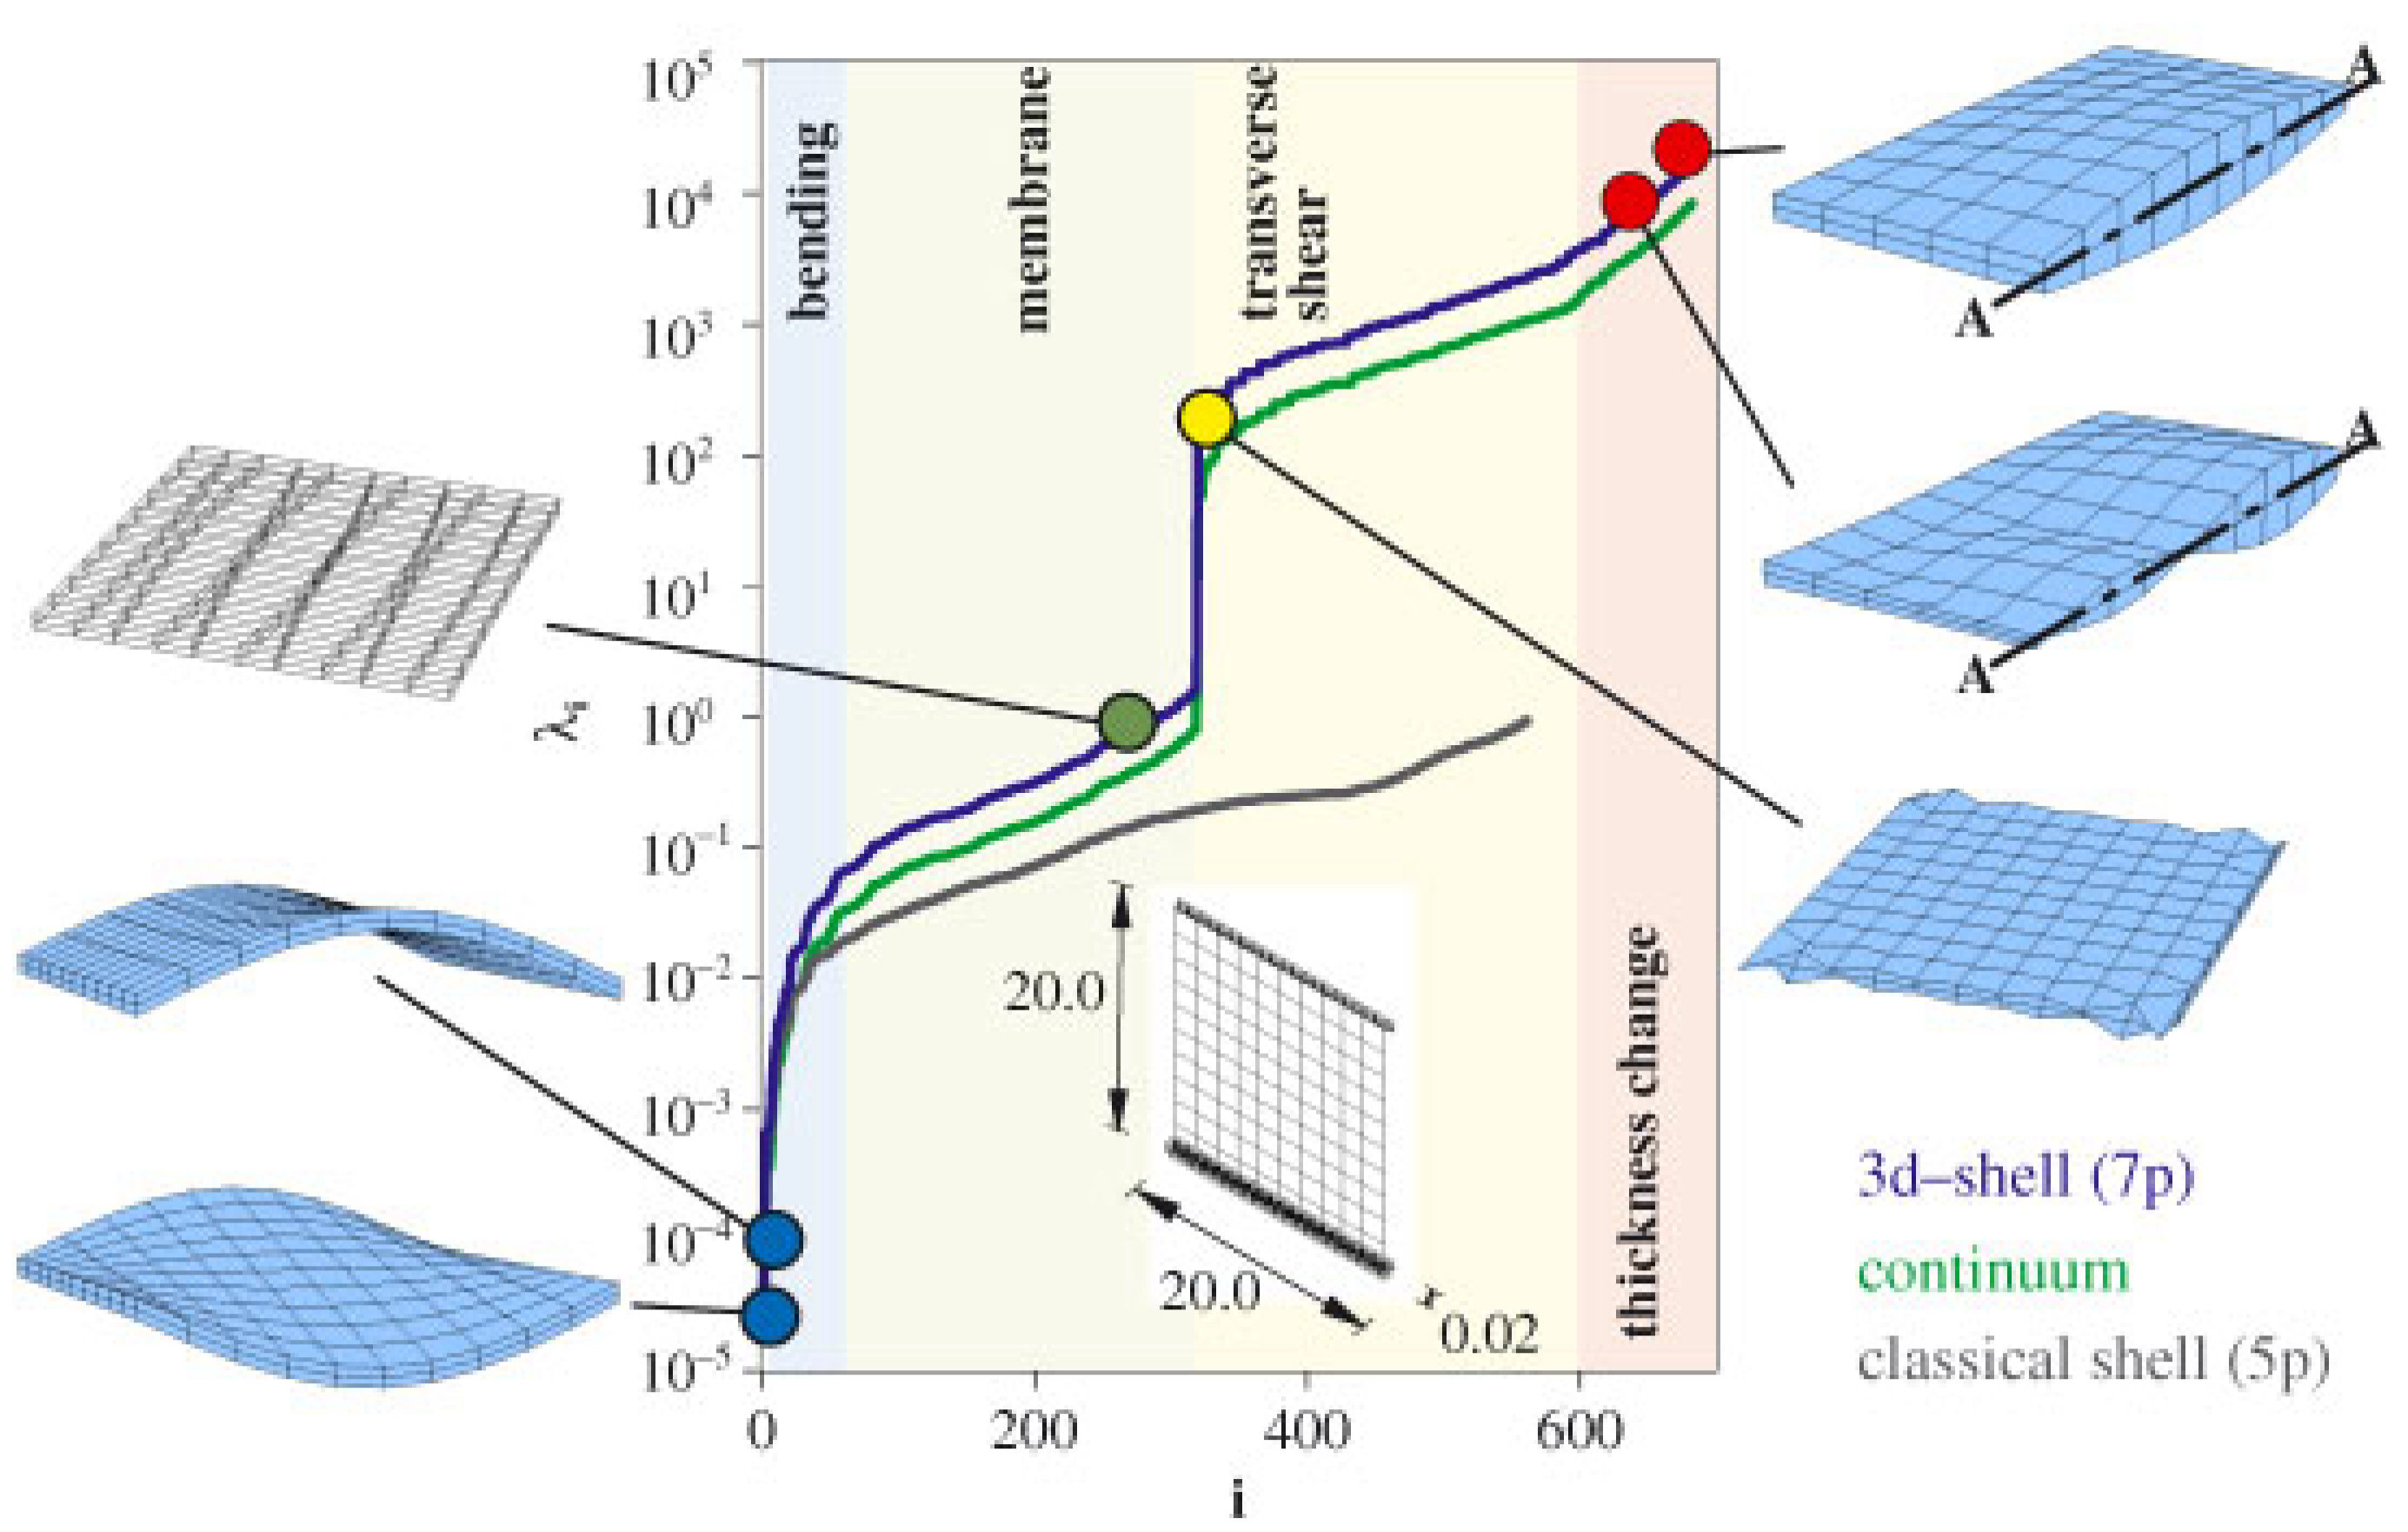
\includegraphics[width=12cm]{images/eigenvaluespectra.png}
	\caption{Eigenvalue spectra of various shell models \cite{RammLitBook04}}
	\label{shelleigenvaluespectra}
\end{figure}

As expected, the 7 parameter model captures higher Eigen-frequencies associated with thickness modes, while the 5 parameter is unable to resolve these. This is yet another example of model selection limiting the possibility of phenomena resolved.

\section{Locking in shell finite elements}

Surveying a range of shell models has confirmed that not all of them are appropriate for every type of analysis. One must consider the capabilities of the model in conjunction with the supposed critical phenomena of the analysis at hand. Thus, the analysis results are a function of physics the shell model can \textit{express}. This concept of expression limitation is vital to the correct understanding of shells in the FEM. If the isogeometric approach to the FEM is employed, the field of quantities in the problem are interpolated between discrete nodal values $\hat{(\ )}$ using shape functions $\mathbf{N}$. In general:

\begin{equation} 
\begin{pmatrix}
\mathbf{R} \\
\mathbf{v} \\
\epsilon_{ij} \\
\vdots
\end{pmatrix}
(\xi,\eta)
=
\sum_{m=1}^{n\ nodes}
N(\xi,\eta)_m
{\begin{pmatrix}
	\hat{\mathbf{R}}_m \\
	\hat{\mathbf{v}}_m \\
	\hat{\epsilon_{ij}}_m \\
	\vdots
	\end{pmatrix}}
\label{eqfemtech1}
\end{equation}

The resolving power of the shape functions undoubtedly restricts what continuous fields can be described from discrete values. They govern not only the description of geometry, but also the deformation modes the element can express. This forms another layer of expression limitation added to shell models in FEM. Given the propensity to use linear or quadratic shape functions in modern FEM codes, these limitations are often not insignificant. These, together with the physics assumptions and limitations of each shell model, give rise to common numerical inaccuracies, generally termed locking.

\subsection{Transverse shear locking} \label{transverse_shear_locking}

Transverse shear locking is perhaps the most recognized and problematic locking phenomena amongst the three considered in this work. As it is related to transverse shear strains, transverse shear locking is possible  in the 5 parameter model and impossible for membrane and 3 parameter models. Phenomenologically, transverse shear locking occurs when thin shells incorrectly described by a 5 parameter model are subject to bending situations, with the signature of significantly reduced displacements (ie. 'locked') than expected. By indicating specific material matrices, and removing membrane work for clarity, the internal bending and shear virtual work of the 5 parameter model can be expressed as follows: 


\begin{equation} 
\bar{\mathbf{C}} =
\begin{pmatrix}
1 & \nu & 0 \\
\nu & 1 & 0 \\
0 & 0 & \frac{1-\nu}{2}
\end{pmatrix}
\hspace{10mm}
\mathbf{C}_{bend} = \frac{E t^3}{12(1-\nu^2)} \bar{ \mathbf{C}}
\hspace{10mm}
\mathbf{C}_{shear} = \alpha G t \mathbf{I}
\label{eqlock1}
\end{equation}

\begin{equation} 
-( \delta\Pi_{int} - \delta\Pi_{int\ mem} )=
-(\Pi_{bend} + \Pi_{shear}) =
\int_\Omega
\boldsymbol{\kappa}
:
\frac{E t^3}{12(1-\nu^2)} \bar{ \mathbf{C}}
:
\delta \boldsymbol{\kappa}\ 
d \Omega\ 
+
\int_\Omega
\boldsymbol{\gamma}
:
\alpha G t \mathbf{I}
:
\delta \boldsymbol{\gamma}\ 
d \Omega
\label{eqlock2}
\end{equation}



As phenomenologically described, transverse shear locking comes into effect with thin shells. One can see that as $t \rightarrow 0$ the bending internal work ($\Pi_{bend} \propto t^3$) will be far less than the shear internal work ($\Pi_{shear} \propto t$), leading to an incorrect allocation of internal energy. Since the bending internal work is associated with bending deflections, these resulting deflections will be less than they should be and the element will appear locked. The over-representation of shear strains also leads to strong shear force oscillations - another classic symptom of transverse shear locking.

\subsection{Membrane locking}
\label{membrane_locking_theory}

Membrane locking is the inability to undergo inextensional bending deformations without parasitic membrane contributions. Physically, a primary symptom of this is significantly reduced deformations under pure bending action. Element curvature is a necessary condition for membrane locking, while increasing slenderness exacerbates the problem. Similar to transverse shear locking, as $t \rightarrow 0$ the bending internal work ($\Pi_{bend} \propto t^3$) reduces at a far greater rate than the membrane internal work ($\Pi_{mem} \propto t$) leading to artificial membrane contributions. Thus, membrane locking is possible in 3, 5, and 7 parameter models. The following figure illustrates the increasing severity of membrane locking as slenderness increases for 3 and 5 parameter NURBS based shell models.

\begin{figure}[H]
	\centering
	\def\svgwidth{\columnwidth}
	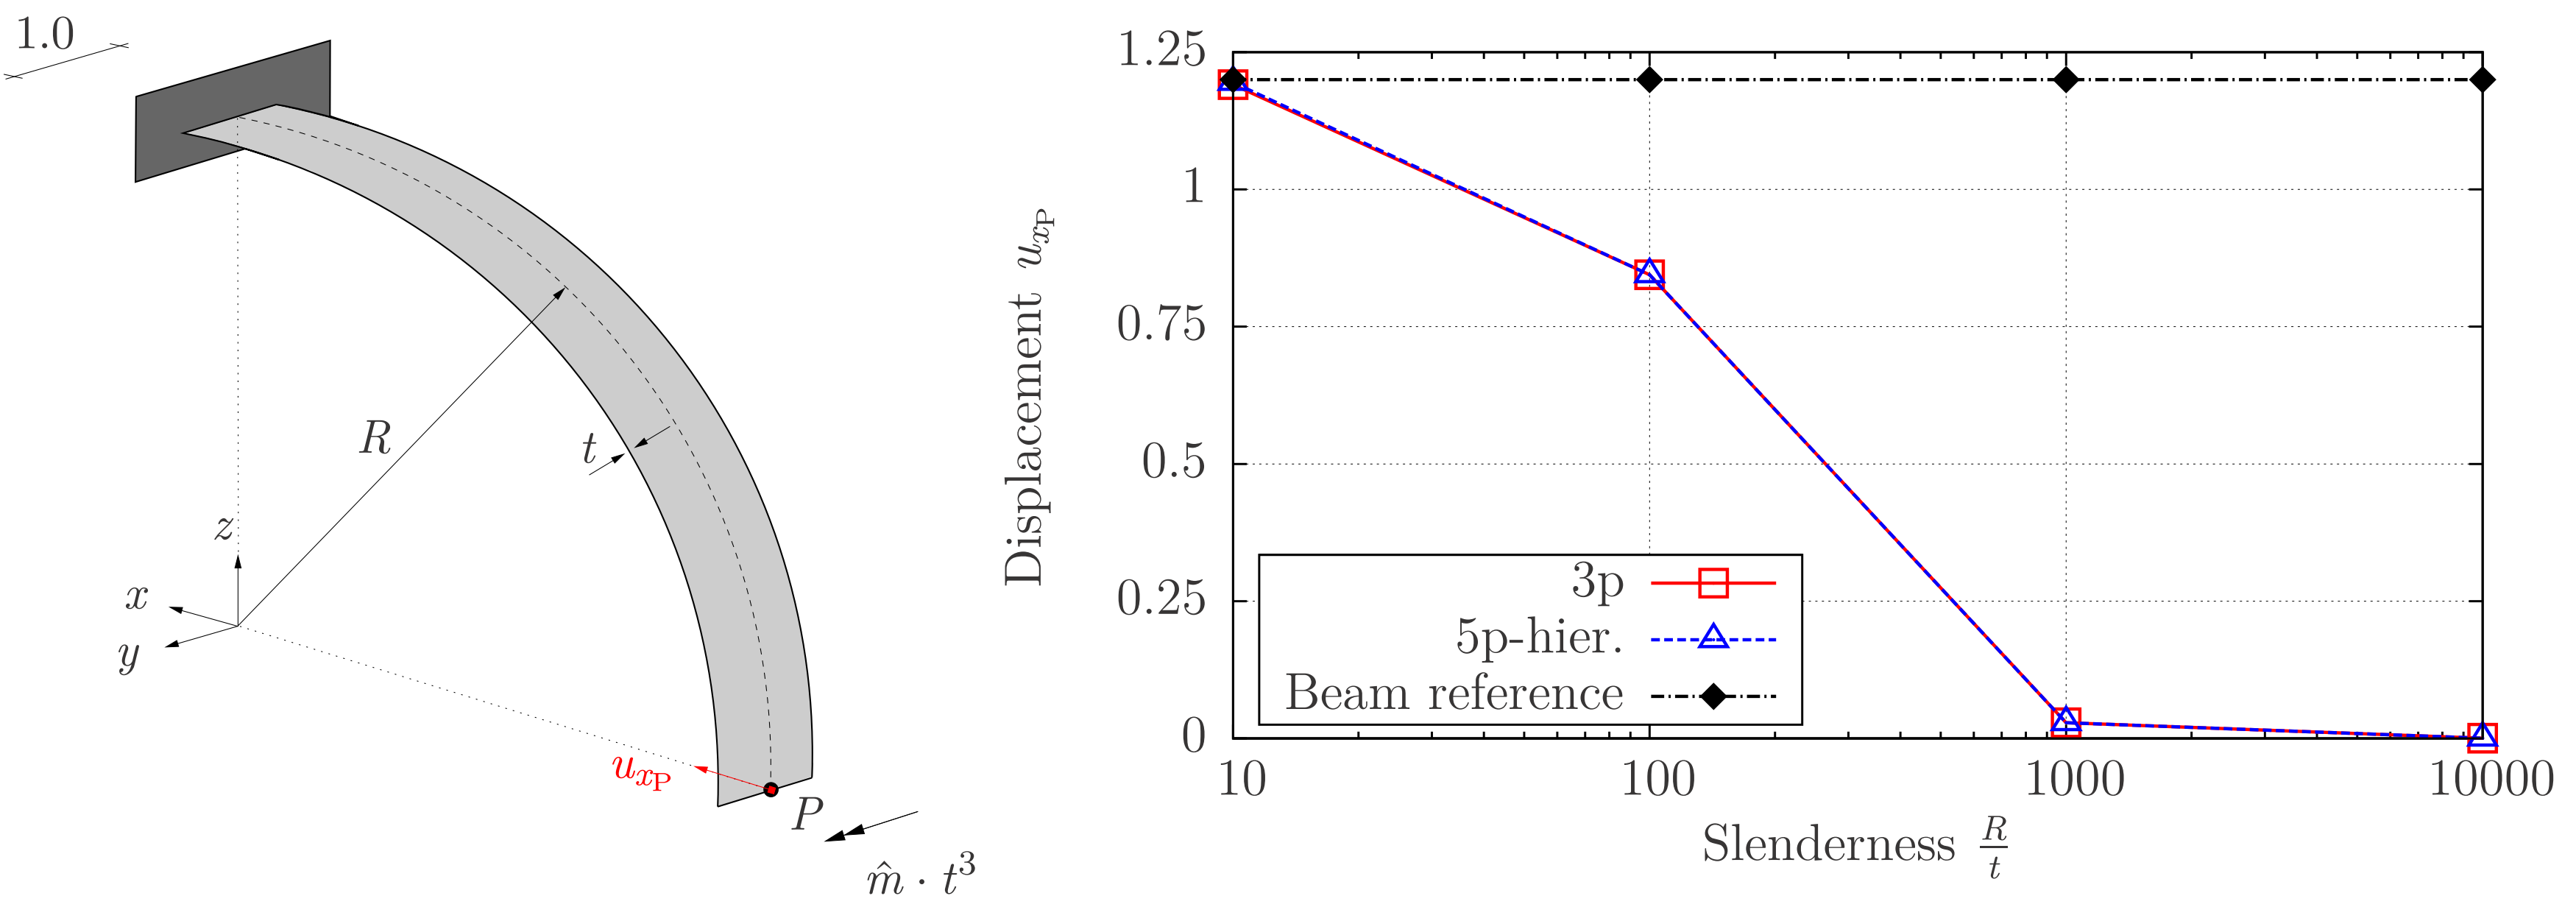
\includegraphics[width=14cm]{images/membranelocking.png}
	\caption{Convergence of cylindrical shell problem demonstrating membrane locking \cite{Echter13}}
	\label{ansexample}
\end{figure}

Despite the bleak results of the above problem, especially in high slenderness range, Bischoff et al. \cite{BischLitBook04} suggest that the adverse effects of membrane locking are mild when using bilinear shape functions, and completely ignored in linear triangle elements (where curvature is always zero). These lower order finite elements form the bulk of what used in commercial FEM codes and are the focus of this work.

\subsection{Curvature thickness locking}

Curvature locking is another locking consideration that only occurs in curved structures with 7 parameter models. The hallmark of curvature thickness locking is artificial through-thickness strains $\epsilon_{33}$ under pure bending action. Since the focus of this work is 3 and 5 parameter models that don't include normal strains $\epsilon_{33}$, the reader is referred to Bischoff et al. \cite{BischLitBook04} and Echter \cite{Echter13} for further information.

\section{Shell finite element technologies}
\label{FE_tech}

The previous discussion of locking phenomena associated with pure displacement formulations of shell finite elements has given rise to a number of shell finite element technologies to improve element performance. Broadly speaking, these mitigation approaches fall into two categories: reduced integration and B-Bar ($\bar{\mathbf{B}}$) approaches which modify the strain displacement matrix $\mathbf{B}$. 

\subsection{Reduced integration}

One of the simplest and oldest methods of curbing locking is reduced integration, which deliberately uses less Gauss points than required to integrate the element stiffness matrix. Typically implemented as selective reduced integration (SRI), where the bending component is fully integrated and only the shear part undergoes reduced integration, the efficacy of the method relies on how susceptible the reduced integration Gauss point locations are to parasitic strains. Despite this 'chance' aspect, it is often used in crash worthiness simulations with the benefits of reduced locking and reduced computational time. The following graph compares the performance (scaled displacement vs. slenderness) of a fully and reduced integrated 5 parameter shell against the reference solution for a square plate in bending.

\begin{figure}[H]
	\centering
	\def\svgwidth{\columnwidth}
	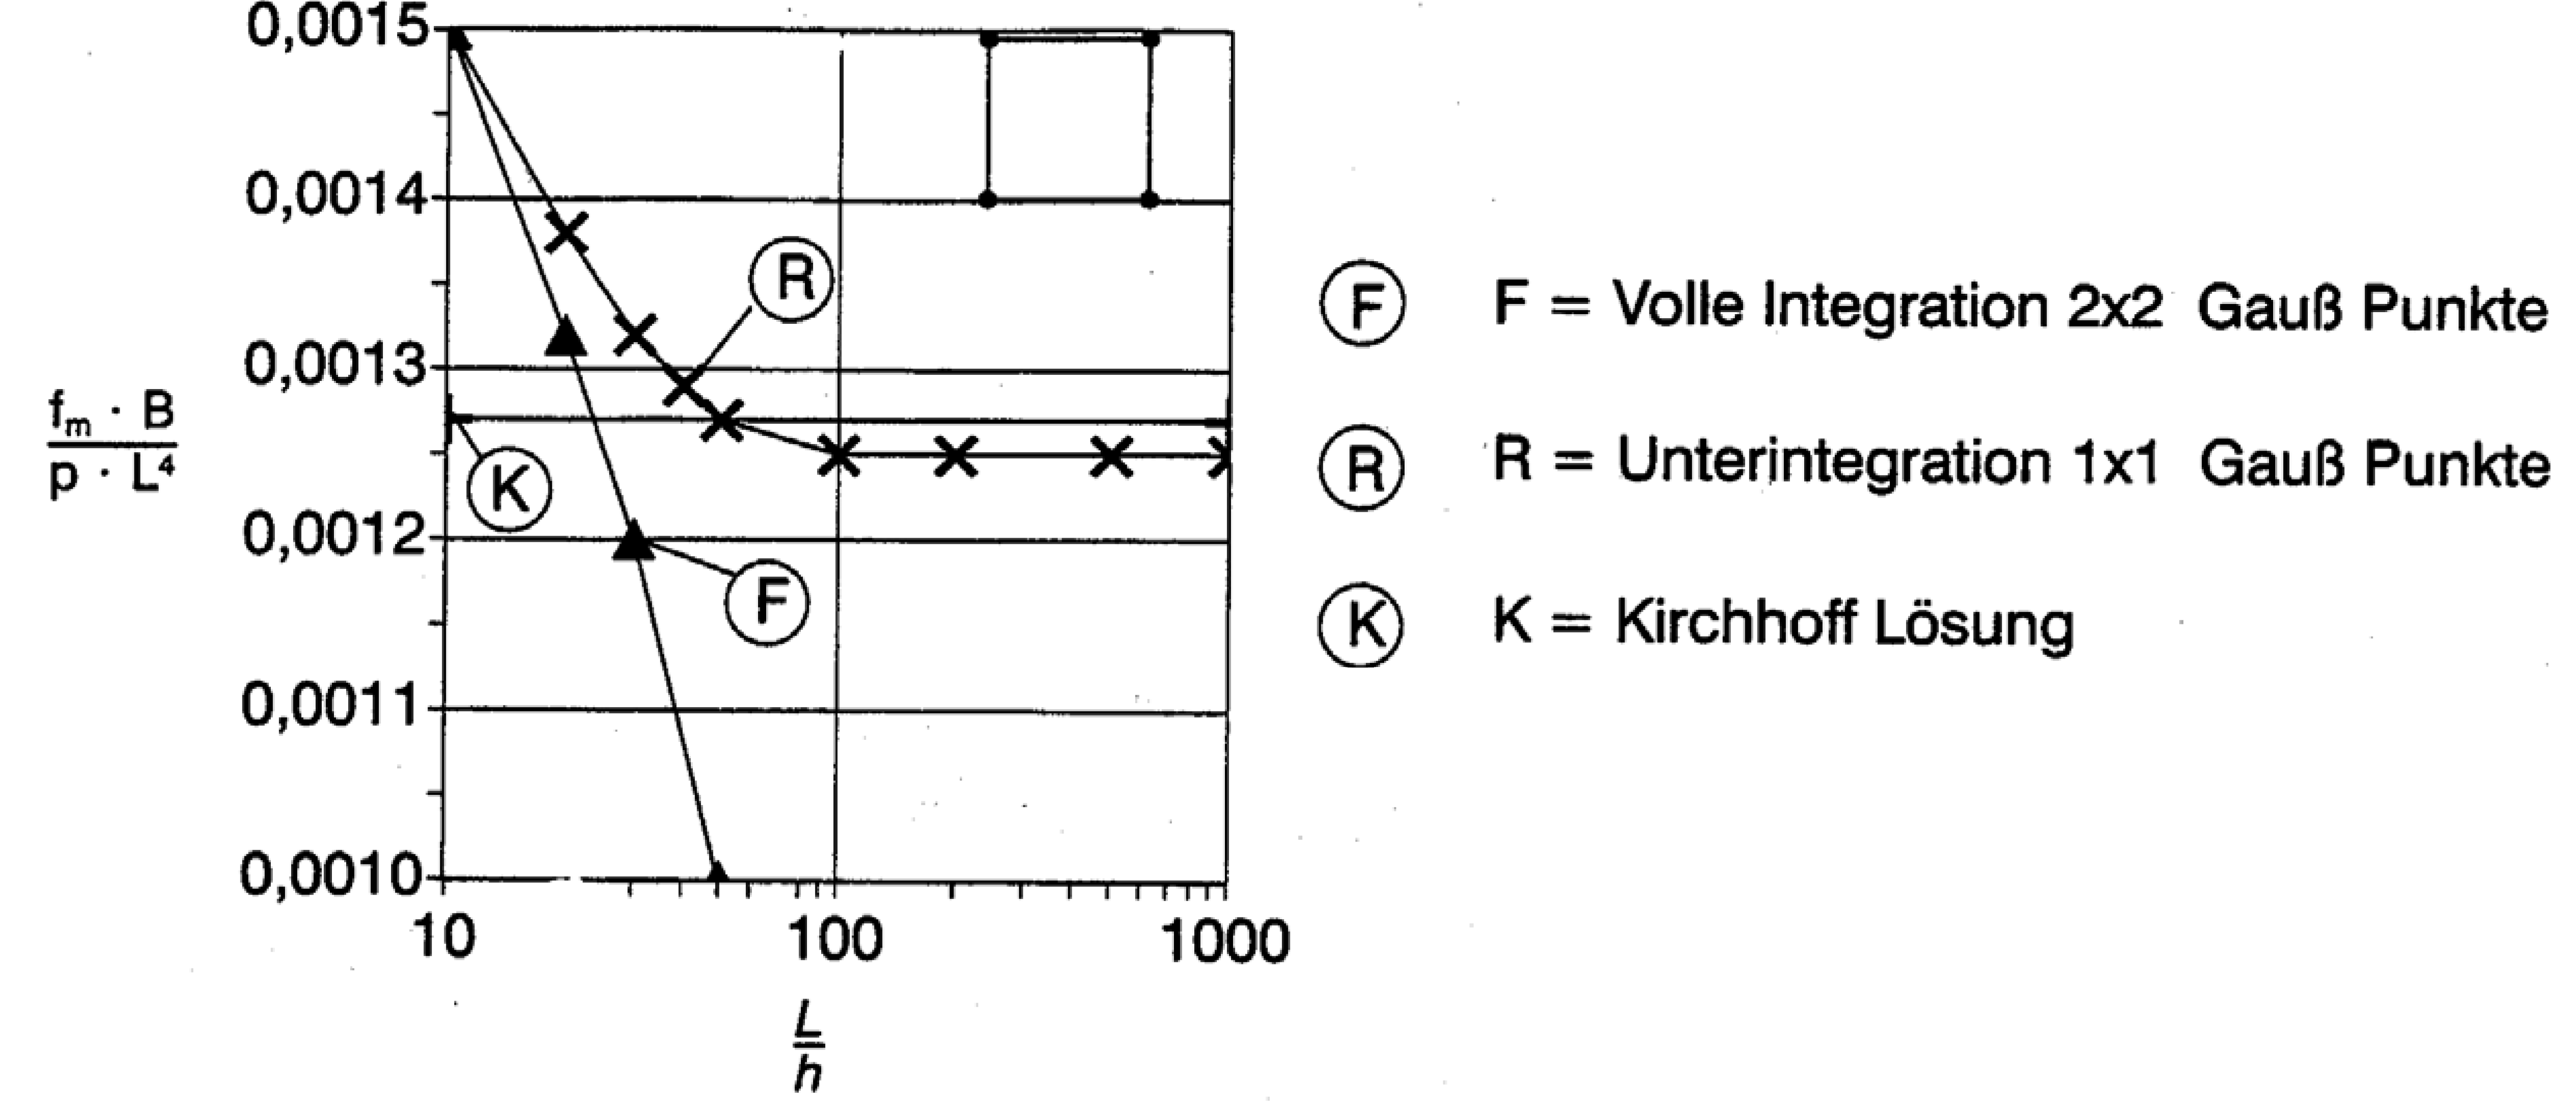
\includegraphics[width=14cm]{images/shearlockingredint.png}
	\caption{Reduced integration of a 5 parameter Quad 4 shell \cite{Bletz16}}
	\begin{flushleft}
	{\scriptsize \textit{F = Full integration, R = Reduced integration, K = Kirchhoff (3 parameter model) solution}}
\end{flushleft}	
	\label{shearlockingredint}
\end{figure}

It's clear that the normal fully integrated element exhibits severe locking, while the element with reduced integration converges to a value close to the reference solution. Despite this, SRI in general still doesn't guarantee complete removal of shear locking and also introduces spurious zero energy modes. These zero energy modes are often combated by stabilizing matrices ("hourglass" control \cite{Zien2Vol2000}) which are designed to be activated under the spurious zero-energy regimes and noted as quite complex to formulate \cite{Mohan97}. An additional drawback of reduced integration is element performance deterioration as the mesh becomes distorted and warped \cite{Nguyen2009} \cite{Yang2000}.

\subsection{Assumed Natural Strains}

The Assumed Natural Strain (ANS) approach forms a main umbrella of B-Bar methods, which alters the strain-displacement matrix $\mathbf{B}$ to mitigate locking. The ANS approach \cite{MACNEAL1982} works by computing the strain values at particular co-location points less susceptible to parasitic strains in the element (normally chosen as mid-edge and/or centre points) and then interpolating these discrete values through the element to define a new "assumed" shear strain field. As a general approach, many subsequent technologies fall under the ANS umbrella.

\subsection{Mixed Interpolation of Tensorial Components}

Falling within the ANS framework, Dvorkin and Bathe \cite{Dvorkin84} \cite{Bathe86} developed the Mixed Interpolation of Tensorial Components (MITC) approach which relies on an assumed shear strain field. A graphical example of this formulation is demonstrated below on a Quad 4 element, with linear interpolation of the shear strain field at mid-side points.

\begin{figure}[H]
	\centering
	\def\svgwidth{\columnwidth}
	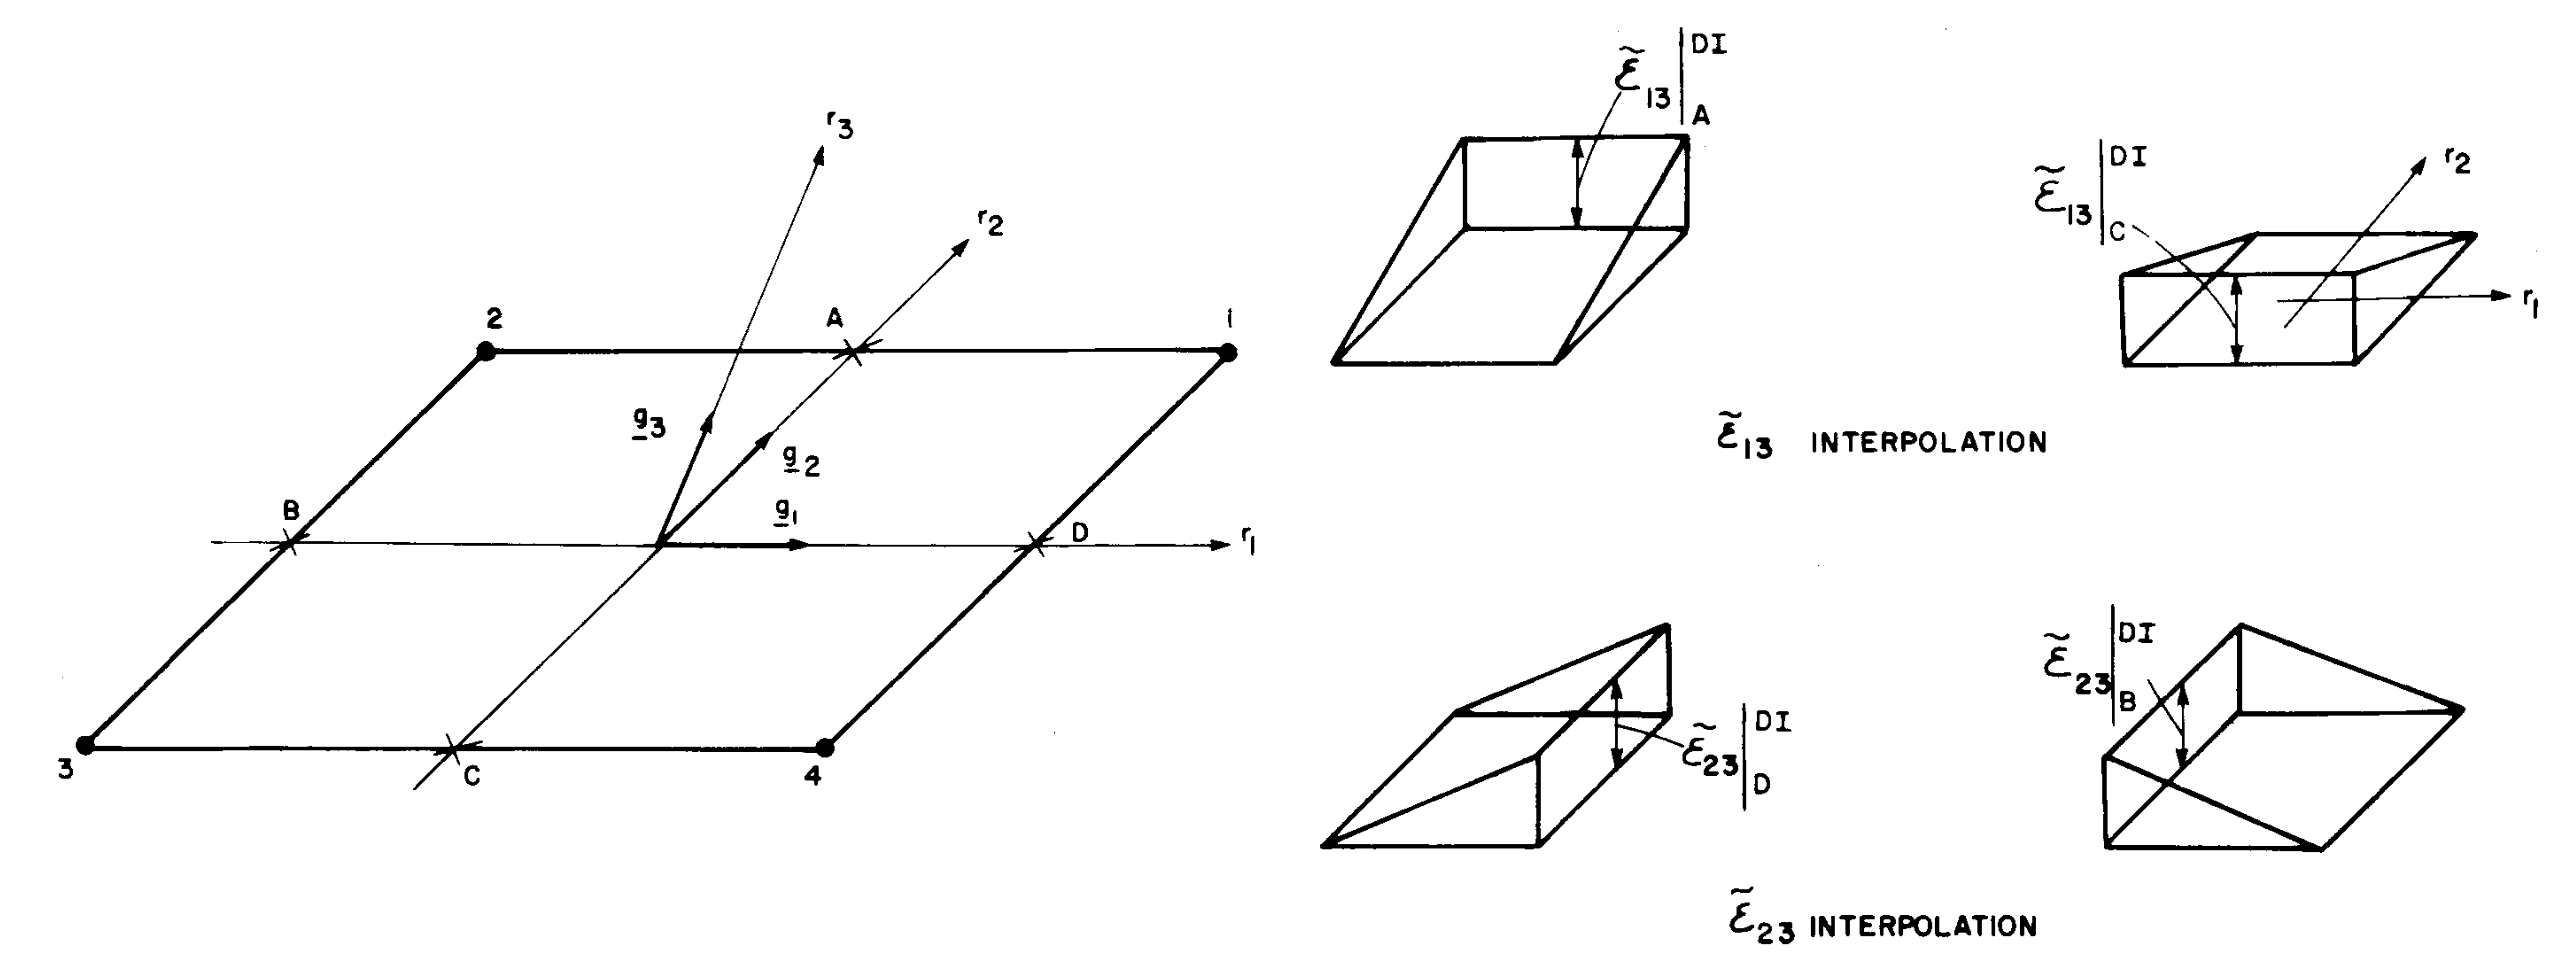
\includegraphics[width=16cm]{images/mitc4.png}
	\caption{Assumed shear strain field of the MITC4 element \cite{Bathe86}}
	\label{ansexample}
\end{figure}

The performance of the MITC formulation clearly depends on the location of the sampling points, and their susceptibility to parasitic shear strains under the case considered. Despite this, the MITC elements have proven resistant to membrane and transverse shear locking \cite{Bathe86} and are amongst the most widely used elements throughout FEM codes.

\subsection{Assumed Natural Deviatoric Strains}

The ANS approach was extended into Free Formulation (FF) \cite{Bergan84}, where the element stiffness matrix is the sum of a basic and higher order stiffness, by Militello and Felippa \cite{FELIPPA1990} under the name of the Assumed Natural Deviatoric Strains (ANDES) formulation. An advantage that the ANDES formulation inherits from the FF is that it untethers the derivation of element stiffness from the principle of minimum potential energy, the function continuity requirements of which often result in elements that "tend to be too stiff" \cite{Bergan84}. The ANDES basic stiffness ensures consistency of the element and arrises from the basic strain field comprising constant strain states and those associated with rigid body motion. Complementing this, the higher order stiffness is responsible for stability and accuracy \cite{Felippa2003} based on a enhanced strain field where the element enhancements are realised. The FF framework requires this potentially non-conforming higher order field be energy orthogonal to the basic field, which the ANDES formulation fulfils with a deviatoric higher order strain field \cite{felippa2002fitting}.  The ANDES formulation has proven capable of alleviating membrane and transverse shear locking \cite{Mostafa11}.

\subsection{Discrete Shear Gap}

The Discrete Shear Gap (DSG) approach from Bischoff and Bletzinger \cite{Ble00} \cite{Bis04} is another variant on the ANS approach with the novelty of identifying and manipulating the 'shear gap' field of the element. The shear gap, as illustrated below, is the increase of displacement due to shear, and corresponds to the difference between the actual displacement and that of pure bending (thus the shear gap is always zero in a 3 parameter Kirchhoff-Love model).

\begin{figure}[H]
	\centering
	\def\svgwidth{\columnwidth}
	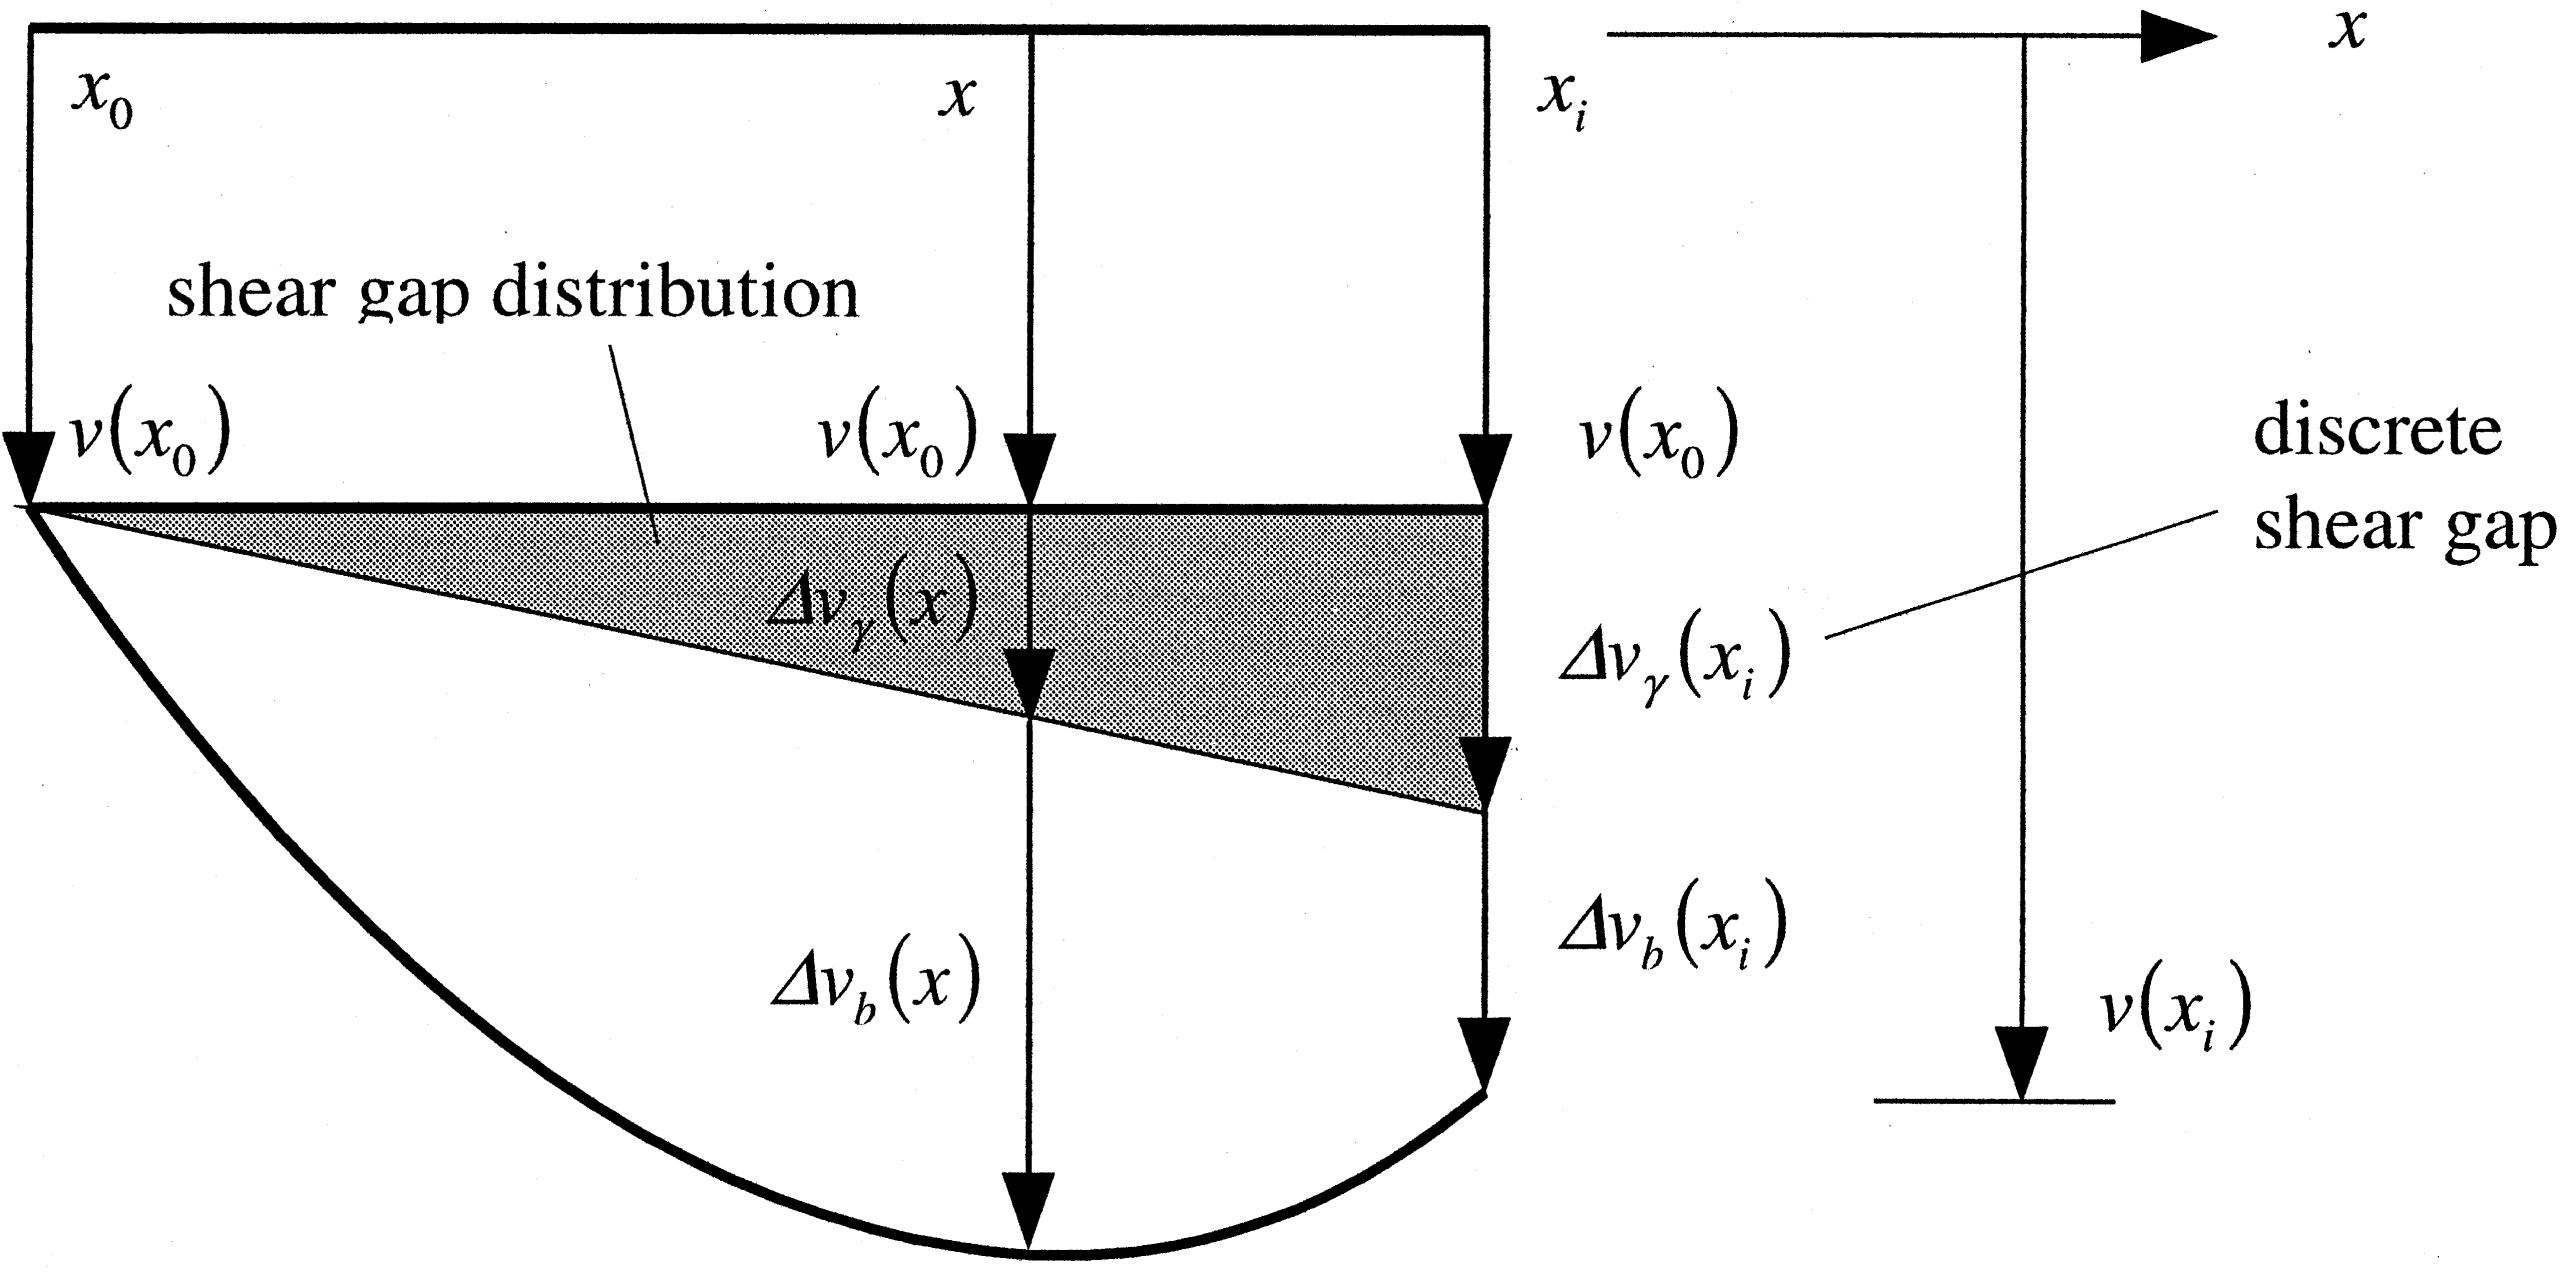
\includegraphics[width=8cm]{images/DSG.png}
	\caption{Discrete Shear Gap (DSG) concept \cite{Ble00}}
	\label{ansexample}
\end{figure}

The DSG method aims to set the nodal shear gaps to zero, which, in effect, alters and defines the underlying shear strain field. In bilinear rectangular applications of the DSG method, Bletzinger \cite{Ble00} notes that the MITC4 element is recovered. For a linear triangle element, the shear gap of only two nodes can be set to zero, rendering the element stiffness dependent on node ordering \cite{Ble00}. Despite this drawback, which diminishes with mesh refinement, the DSG method offers an advantage of very fast computational construction of element stiffness matrices and effective mitigation of transverse shear locking.

\subsection{Discrete Kirchhoff Theory}
\label{dkqtheory}

Elements based on the Discrete Kirchhoff Theory (DKT) are obtained by modifying a basic 5 parameter element and ignoring the transverse shear energy \cite{Batoz1980}. Since the underlying kinematics of the 5 parameter model are different to Kirchhoff bending theory, the Kirchhoff constraints are enforced via discrete points (typically nodes and mid-edge points) along the element edges relating the rotations to translational displacements. The geometry and tying-points of the Discrete Kirchhoff Quadrilateral (DKQ) element are shown below:

\begin{figure}[H]
	\centering
	\def\svgwidth{\columnwidth}
	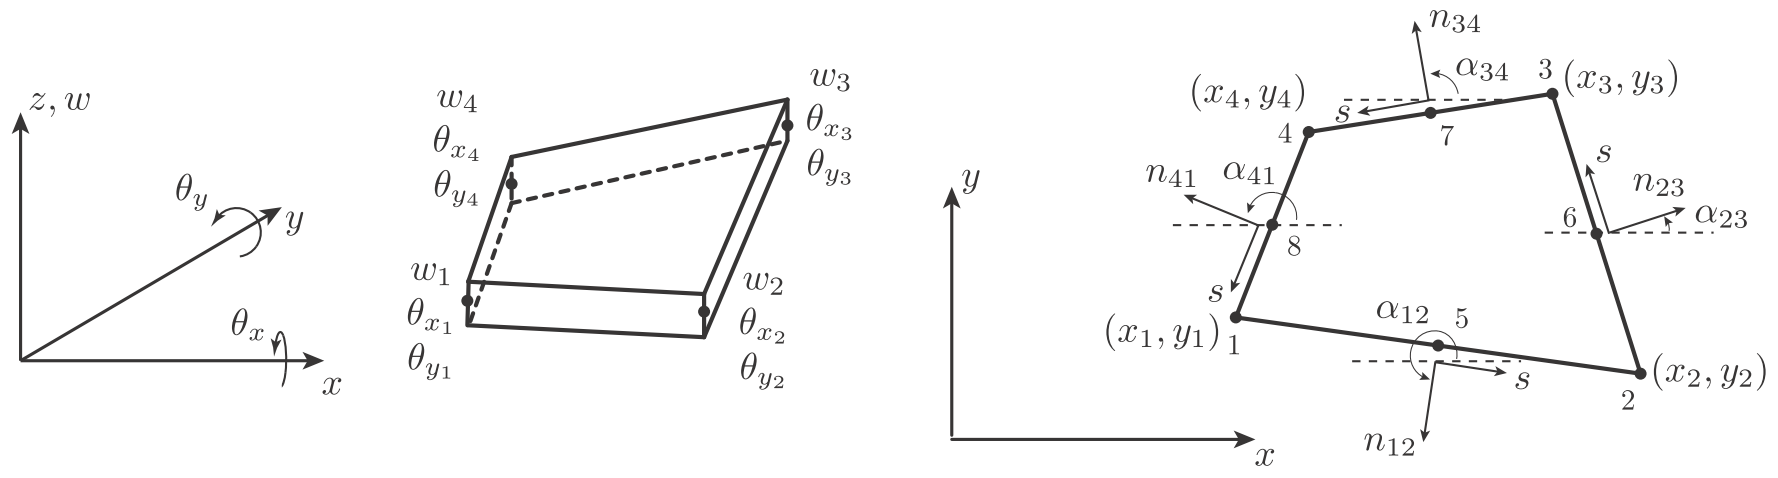
\includegraphics[width=15cm]{images/8nodeseren.png}
	\caption{DKQ DOF arrangement and geometry \cite{Bar12}}
	\label{DKQlayout}
\end{figure}

For example, the Kirchhoff conditions are imposed at corner nodes $i = 1, 2, 3, 4$ and mid-side nodes $k = 5, 6, 7, 8$ \cite{Bar12}:

\begin{equation} 
\beta_{xi} + \frac{\partial w}{\partial x} \rvert_i = 0\ ,
\hspace{10mm}
\beta_{yi} + \frac{\partial w}{\partial y} \rvert_i = 0\ ,
\hspace{10mm}
\beta_{sk} + \frac{\partial w}{\partial s} \rvert_k = 0
\label{eqsdkt}
\end{equation}

Mohan \cite{Mohan97} noted that a major drawback of DKT elements is that the transverse displacement isn't explicitly defined within the interior of the element. Despite this, the advantages of DKT formulated elements is that they combine the shear locking free performance of KL models and the lower $C_0$ continuity requirements of RM models \cite{Bletz16}.

\subsection{Enhanced Assumed Strains}

The Enhanced Assumed Strain (EAS) approach \cite{Simo1990} utilises the three field Hu-Washizu variational principle which allows the simultaneous variation of displacements, stresses and strains. Unlike the other technologies presented which attempt to remove problematic strain terms associated with locking, EAS derived elements feature additional enhanced strain fields designed to balance the parasitic displacement based strain terms. To prevent singular matrices the enhanced strains must be linearly independent from the displacement based strains. Furthermore, orthogonality of the stress functions to the enhanced strains must be ensured such that the associated energy vanish \cite{Echter13}. The application of EAS techniques to elements has been found to improve transverse shear and membrane locking performance \cite{Simo1990} \cite{BischLitBook04} \cite{Echter13}.

\subsection{Drilling degrees of freedom} \label{drilling_DOF_section}

Although drilling degrees of freedom (DOFs) don't counter locking problems, it is a commonly employed finite element technique. The common analysis of structural connections and custom steelwork are instances where shell elements will intersect with each other at arbitrary orientations. The discussion of 3 and 5 parameter shell models confirmed the nodal DOFs to be 3 translation and 2 rotational components:

\begin{equation} 
\mathbf{v}_i^T = \begin{pmatrix}
v_{xi} & v_{yi} & v_{zi} & \beta_{xi} & \beta_{yi}
\end{pmatrix}
\label{eqsdrilling}
\end{equation}

It can be seen that the shell formulations don't require a rotational DOF around the z axis $\beta_{zi}$, referred to as the drilling DOF. However, as discussed, shell elements in practical FEA may meet at arbitrary orientations, such as the perpendicular intersection below:

\begin{figure}[H]
	\centering
	\def\svgwidth{\columnwidth}
	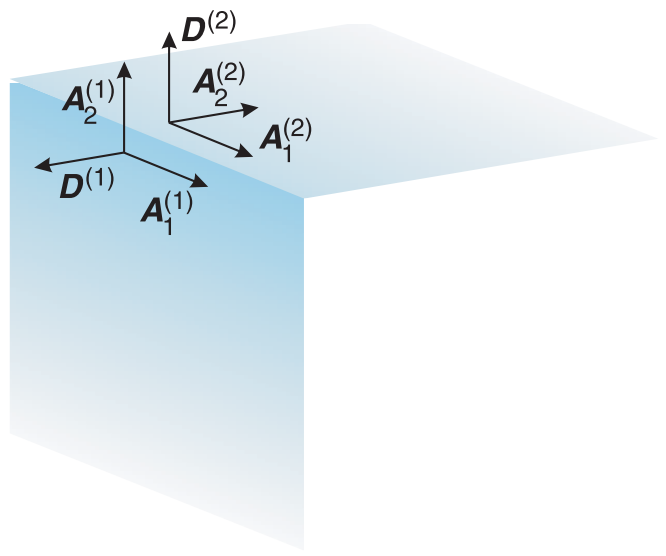
\includegraphics[width=8cm]{images/drillingDOF.png}
	\caption{Shell assembly benefitting from drilling DOFs \cite{BischLitBook04}}
	\label{shellModels}
\end{figure}

The figure above illustrates that the real twisting DOF associated with $A_2^{(2)}$ mates with the drilling DOF associated with $D^{(1)}$, which has no theoretically based stiffness value according to the shell formulations. In the current arrangement the connection will clearly be modelled too flexibly.  A remedy for this is the addition of an artificial drilling DOF stiffness to the element, however the magnitude of such a fictitious torsional spring has no decisive theoretical foundation. Intuitively, it should be done on an element by element basis and should vary with the characteristic size and stiffness of the element, as opposed to a global constant drilling stiffness. Among others available, one common technique is to introduce a scaling factor (in the strain-displacement matrix or after the element stiffness matrix is constructed) which takes a fraction of the element stiffness and assigns it to the drilling DOFs. 

\subsection{Summary of selected element technologies}

Following the discussion of shell models, their associated locking phenomena and element technologies, a summary of the element technologies considered with their relative merits and drawbacks is tabulated below:

\begin{table}[H]
	%\singlespace
	\onehalfspacing
	\begin{tabularx}{\textwidth}{ | l | l |  X | X | }
		\hline
		\textbf{Technology} 		& 	\textbf{Formulation}	&		\textbf{Advantages}	&		\textbf{Disadvantages}\\
		\hline
		ANDES	& 5 parameter &	Reduced membrane and transverse shear locking &  Locking reduction depends on tying points \\
		\ &\  & Relaxed higher order strain field & More complex implementation \\
		\hline
		ANS & 5 parameter		&  Reduced membrane and transverse shear locking & Locking reduction depends on tying points \\
		\hline
		DKT	&  3 parameter		 & 	No transverse shear locking & Transverse disp. not explicitly defined \\
		\hline
		Drilling DOFs	  &  - & Practical assembly of shells & Artificial stiffness \\
		\hline
		DSG	&	 5 parameter	& Reduced transverse shear locking	& Node numbering dependency for linear triangle \\
		\ &\  & Computationally fast & \  \\
		\hline
		EAS 	  &		  5 parameter		&		Reduced transverse shear and membrane locking & Potentially complex implementation and possibly slower \\
		\hline
		MITC	&		5 parameter	&		Reduced membrane and transverse shear locking & Locking reduction depends on tying points \\
		\hline
		Reduced &		-		&	 Lowered computational cost & Zero energy modes \\
		integration &\  & Reduced locking & Locking reduction depends on integration points \\ 
		\hline
	\end{tabularx}
	\caption{Summary of selected element technologies}
	\label{table:1}
\end{table}

The table above confirms the \textit{"no free lunch"} theory, with every technology having its own advantages and drawbacks. In the case of a flat shell (naturally, or via projection), where the bending and membrane response are decoupled, a single finite element can easily employ different technologies in each component. 

\section{Identification of Kratos shell element formulations}

The shell elements to be implemented in Kratos are the 5 parameter (Reissner-Mindlin theory) triangular shell and the 3 parameter (Kirchhoff Love theory) quadrilateral shell. Obviously the perfect element choices for Kratos would be computationally quick, possess no locking and easy to implement, but it's clear such an element doesn't exist yet. If the requirements are relaxed to computationally quick elements that are relatively free of locking effects the following candidates are selected:

\begin{table}[H]
	\begin{tabularx}{\textwidth}{ | l | X |  X | }
		\hline
		\textbf{Element} 		& 	\textbf{Membrane formulation}	&		\textbf{Bending formulation}	\\
		\hline
		Thick triangular shell
		&
		DSG + Drilling DOFs
		&
		DSG \\
		\hline
		Thin quadrilateral shell
		&
		ANDES including Drilling DOFs
		&
		Discrete Kirchhoff Quadrilateral (DKQ) \\
		\hline
	\end{tabularx}
	\caption{Selected formulations of implemented shell elements}
	\label{table:2}
\end{table}

With the various components of the KRATOS shell elements selected, they shall be implemented in the following sections of this work, commencing with the DSG triangle element.